\chapter{Signal fit}
\label{sec:Signalfit}
This chapter describes the way how the yield \NDp of the signal decays \LbToDpmunuX is determined.
Due to the missing neutrino, the reconstructed \Lb mass does not peak at its actual mass and cannot be used to distinguish signal from background.
Nonetheless the \Dz\proton subsystem is of particular interest.
Recently, \babar measured the decay of two \Lc resonances into \Dz\proton, namely \decay{\LcResI}{\Dz\proton} respectively \decay{\LcResII}{\Dz\proton} \cite{BaBar_D0p}.
It is expected, that the \LcResI and \LcResII also appears in the invariant \Dz\proton mass of the decay \LbToDpmunuX through the decay \decay{\Lb}{\LcRes{(2880/2940)}\mun\neumb} with \decay{\LcRes{(2880/2940)}}{\Dz\proton}.
Indeed, there are some peaking structures at \MDp around 2880\mev and 2940\mev as Figure \ref{fig:plot_mD0p_logIP} (top) shows.
As a nice side effect, the masses and widths of those resonances can be determined, too.
However, it is expected that most of the \LbToDpmunuX decays are nonresonant, i.e. they decay directly into the $\Dz\proton\mun\neumb X$ final state without going through an intermediate resonance.
It should be stressed, that the measurement of \BR(\LbToDpmunuX) is an inclusive measurement.
This means, that every decay of a \Lb into a final state including a \Dz\proton\mun\neumb is considered as signal.
Thus, the nonresonant \Lb decays as well as the decays via the \LcResI and \LcResII resonances are counted to the signal yield \NDp.

Unfortunately, the nonresonant \Lb decays cannot be disentangled in the \Dz\proton mass from combinatorial background like \BToDmunuX with randomly combined protons.
As already mentioned in Section \ref{sec:Backgrounds}, an appropriate discriminating variable between signal and those combinatorial backgrounds is \logIP.
Just to remind, it has been defined as the logarithm of the difference between the \chisqvtx of the \Dz\mun candidate with and without the proton, i.e. $\logIP := \log\left[\chisqvtx(\Dz\proton\mun) - \chisqvtx(\Dz\mun)\right]$.
The smaller \logIP, the better the proton makes a vertex with the \Dz\mun candidate and the more likely it is a \LbToDpmunuX signal event.
Figure \ref{fig:plot_mD0p_logIP} (bottom) illustrates the discriminating power of \logIP when one compares the data and the wrong sign distributions.

The strategy for the signal fit is to perform a two-dimensional binned likelihood fit to the \Dz\proton mass to learn as much about intermediate resonant states as possible and simultaneously to the \logIP distribution to disentangle \LbToDpmunuX signal from combinatorial background.
Unfortunately, there is no theoretical description of the \LbToDpmunuX decay and the distributions of \MDp and \logIP.
Thus, the most important task is to find a proper parametrisation of the two-dimensional distribution on an empirical basis.
Depending on the respective variables either data driven methods or simulations are used for that purpose as will be described in the following section.

% ==================================
% Section: Fit parametrisation
% ==================================
\section{Empiric determination of the shape of the two-dimensional \logIP/\MDp distribution}
This section describes the determination of the shapes for the \logIP distribution and the \Dz\proton mass shape.
Though there will be a two-dimensional fit in the end, it is assumed that the \logIP and \MDp distributions can be determined separately for each fit component.
The two-dimensional fit is rather needed for the separation of the different fit components, for instance the \MDp shapes are very similar for nonresonant signal and background but completely differ in their \logIP shape, i.e. their vertex quality.

For \logIP, the functions to be fitted on data are determined with simulations.
This determination is done for signal and background separately.
Both shapes are then combined and fitted to data.

Concerning the invariant \Dz\proton mass, there do not exist any reliable simulations predicting its shape.
Here it is assumed that the behaviour of the combinatorial background component is similar to the wrong sign events.
Hence, the \MDp distribution of the wrong sign events is used to get the shape of the background component.
The signal component is determined with the data itself.
To highly suppress combinatorial background leaking into the \Dz\proton mass distribution, only events with a $\logIP < 1$ are fitted.
This corresponds to the distribution shown in Figure \ref{fig:plot_mD0p_logIP} (top).

\subsection{\logIP shape}
As already mentioned both, \logIP signal and background components, are determined with simulations.
The \logIP distribution of the signal simulation in Figure \ref{fig:fit_logIP_signal} reminds of a Gaussian curve, but having different widths to the left and the right from the maximum.
Thus, it is parametrised with a so called \textsc{bifurcated Gaussian}.
A bifurcated Gaussian is an asymmetric Gaussian with two different widths for the left and the right part from the maximum.
If $\mathcal{G}(x|x_0,\sigma) = \frac{1}{\sqrt{2\pi}\sigma}\exp\left(-\frac{x-x_0}{2\sigma}\right)$ denotes a usual Gaussian with mean $x_0$ and width $\sigma$, a Bifurcated Gaussian can be written as\footnote{All fitfunctions in the following are given without normalisation factors. That is why there always appears a $\propto$ sign instead of an equal sign.}
\begin{align}
    \text{BfG}(x|x_0, \sigma_{\text{L}}, \sigma_{\text{R}}) \propto 
    \begin{cases}
        \mathcal{G}(x|x_0,\sigma_{\text{L}}) & \text{for } x < x_0 \\   
        \mathcal{G}(x|x_0,\sigma_{\text{R}}) & \text{for } x > x_0 \\   
    \end{cases},
\end{align}
The tails on both sides of \logIP are very broad compared to the peaking part.
Thus a single bifurcated Gaussian is not sufficient.
The final fit function for the signal \logIP shape is the sum of two bifurcated Gaussians, in the following called a double Bifurcated Gaussian DBfG
\begin{align}
    &\text{DBfG}(x|x_0,\vec{\sigmaL{}}, \vec{\sigmaR{}}, f_{\BfG_1}) \propto \nonumber \\
    &f_{\BfG_1} \BfG(x|x_0,\sigmaL{1}, \sigmaR{1}) + \left(1 - f_{\BfG_1} \right) \BfG(x|x_0,\sigmaL{2}, \sigmaR{2}),
\end{align}
where $f_{\BfG_1}$ denotes the fraction of the first \BfG and the two \BfG share a common mean $x_0$. 
The fit result for the signal simulation can be seen in Figure \ref{fig:fit_logIP_signal}.
\begin{figure}[ptb]
    \centering
	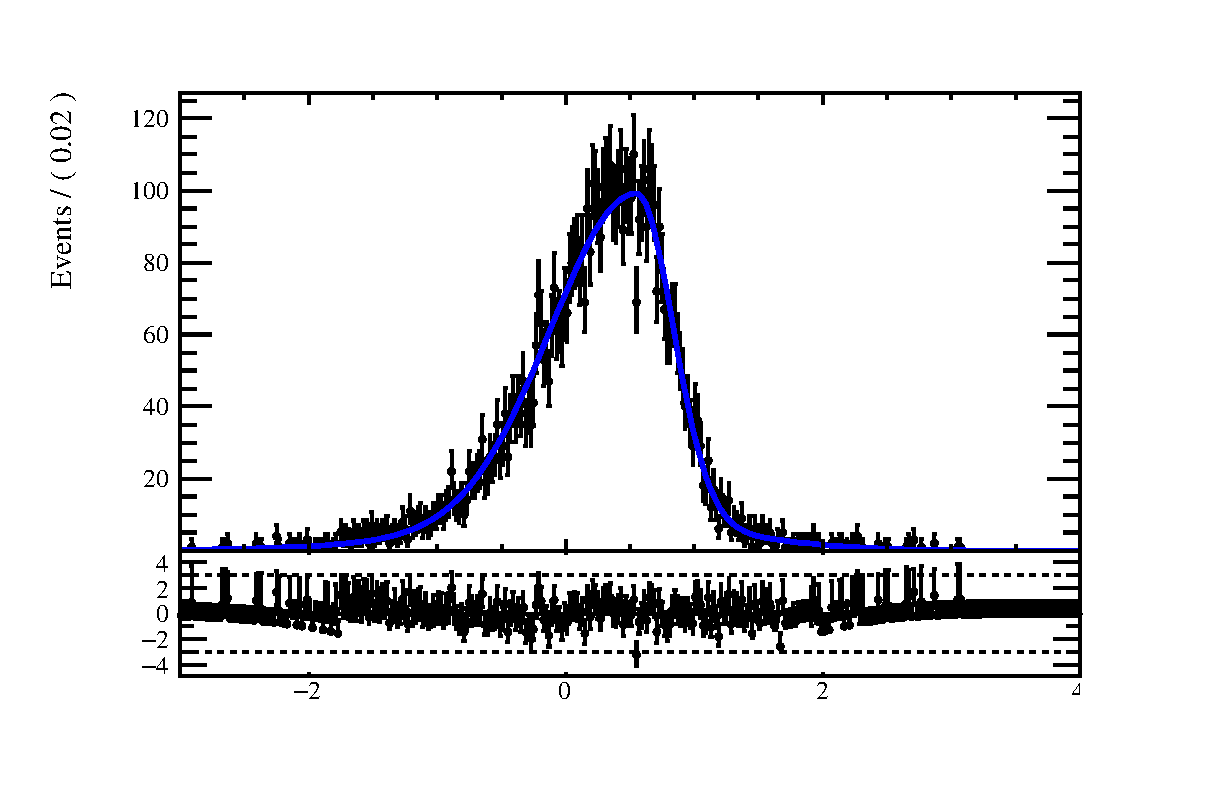
\includegraphics[width=0.75\textwidth]{LbToD0p/fits/MC_D0p_SIG/logIP_RS/fit_DBfG}
	\caption{Fit to the \logIP distribution of the signal simulation. As parametrisation a double Bifurcated Gaussian has been chosen.}
    \label{fig:fit_logIP_signal}
\end{figure}
In order to estimate the quality of the fit, the \textsc{pull} distribution is also shown in Figure \ref{fig:fit_logIP_signal} below the \logIP distribution.
The pull of a variable $x$ is defined as
\begin{align}
    \text{pull}(x) = \frac{N_\text{meas}(x)-N_\text{fit}(x)}{\sigma_{N_\text{meas}}(x)}.  \label{eq:pull}
\end{align}
Referring to Figure \ref{fig:fit_logIP_signal}, $N_\text{meas}(x)$ denotes the number of entries in the bin with $\logIP = x$, $N_\text{fit}(x)$ the corresponding result of the fit in the respective bin and $\sigma_{N_\text{meas}}(x)$ the error on $N_\text{meas}(x)$.
In other words, the pulls are the residuals of the fit normalised to the uncertainty.
If the fit describes the data well, the pull distribution should peak and fluctuate around zero with mean 1 \cite{Pulls}.
From the pull distribution it can be stated that the chosen fit model describes the data well, especially in the tails.
A little bias might be included if on closer looks at the region of $\logIP \approx 0$.

Concerning the \logIP background shape, only a simulation with very little statistics is available.
To get a better idea of the background \logIP shape and to increase statistics, right sign and wrong sign events of this sample have been added.
In this case wrong sign events refers to events with a \Lc\mup in the final state.
Compared to the signal \logIP shape, both, right sign and wrong sign events, describe combinatorial background.
Thus, it is assumed that their \logIP shapes are similar as Figure \ref{fig:plot_logIP_MC_BKG} confirms. 
According to this, the addition of right sign and wrong sign is appropriate to increase statistics in this case.

The \logIP distribution of the background simulation looks lika a Gaussian around the maximum, but has a long tail to lower \logIP values.
That is why a single CrystalBall function is chosen as fit function for the \logIP background shape. 
This function was first used by the CrystalBall collaboration to account for radiative losses in \jpsi or \psitwos decays \cite{CrystalBall}. 
It is defined as 
\begin{align}
    &\CB(x|x_0, \sigma, \alpha, n) \propto
    \begin{cases}
        \exp \left(-\frac{(x-x_0)^2}{2\sigma^2}\right)     & \text{for } \frac{x-x_0}{\sigma} > -\alpha \\
        A \cdot \left(B - \frac{x-x_0}{\sigma}\right)^{-n} & \text{for } \frac{x-x_0}{\sigma} \leq -\alpha
    \end{cases}, \\
    &\text{where} \nonumber\\
    &A = \left(\frac{n}{|\alpha|}\right)^n \exp\left(-\frac{|\alpha|^2}{2}\right), \\
    &B = \frac{n}{|\alpha|} - |\alpha|.
\end{align}
Hence, the CrystalBall function is a Gaussian with an enhanced tail at one side of the maximum, due to the power law for $\frac{x-x_0}{\sigma} \leq -\alpha$.
So $\alpha$ denotes the transition between the Gaussian and the power law tail and $n$ the latter's exponent.

The result of the fit to the background simulation can be seen in Figure \ref{fig:fit_logIP_MC_BKG}.
According to the pull distribution the fit nicely describes the data points.
Nonetheless one has to note that statistics here are very little.
\begin{figure}[ptb]
    \centering
	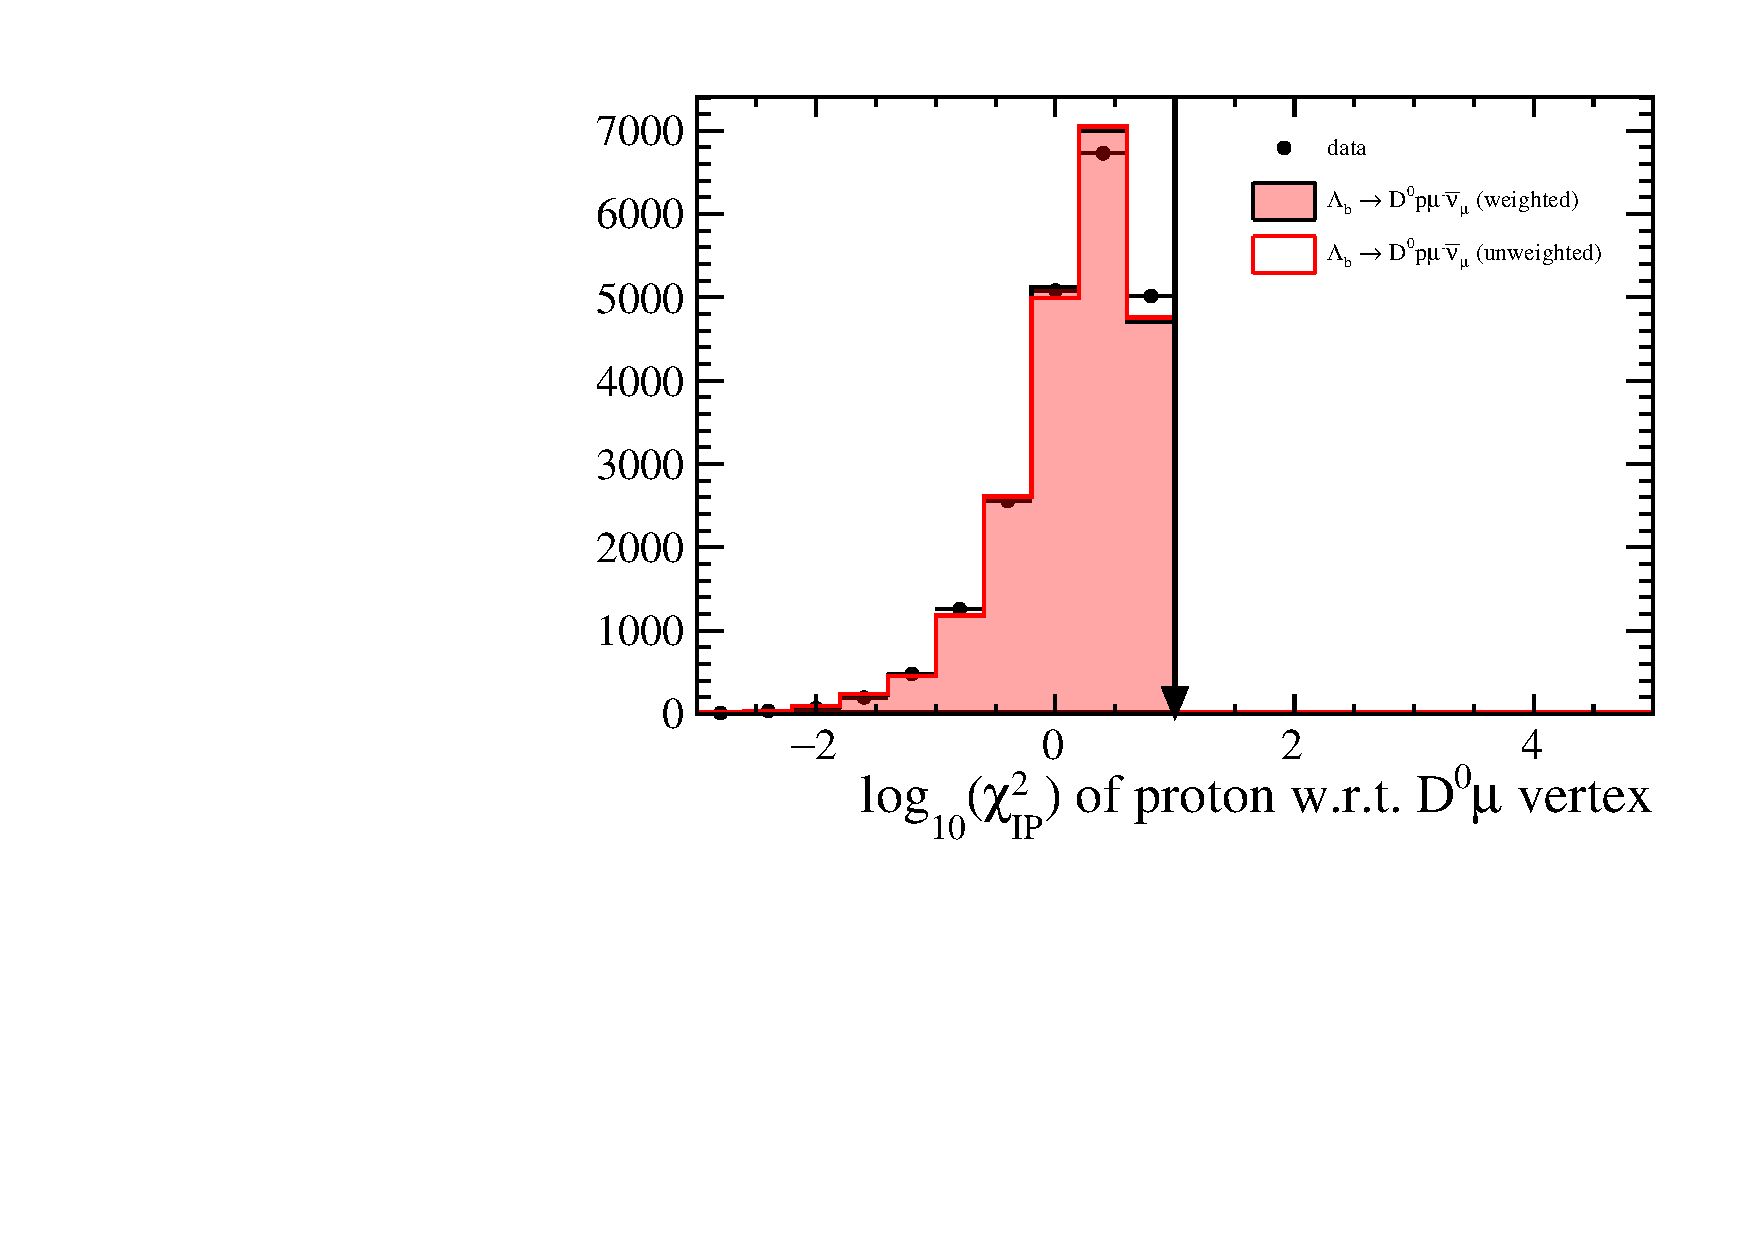
\includegraphics[width=0.75\textwidth]{LbToD0p/plots/MC_B2D0munu_BKG/logIP}
	\caption{Comparison of the \logIP distribution for right sign and wrong sign events in the background simulation. Both, the shapes for right sign and wrong sign are very similar and thus can be added to increase statistics.}
    \label{fig:plot_logIP_MC_BKG}
\end{figure}
\begin{figure}[ptb]
    \centering
	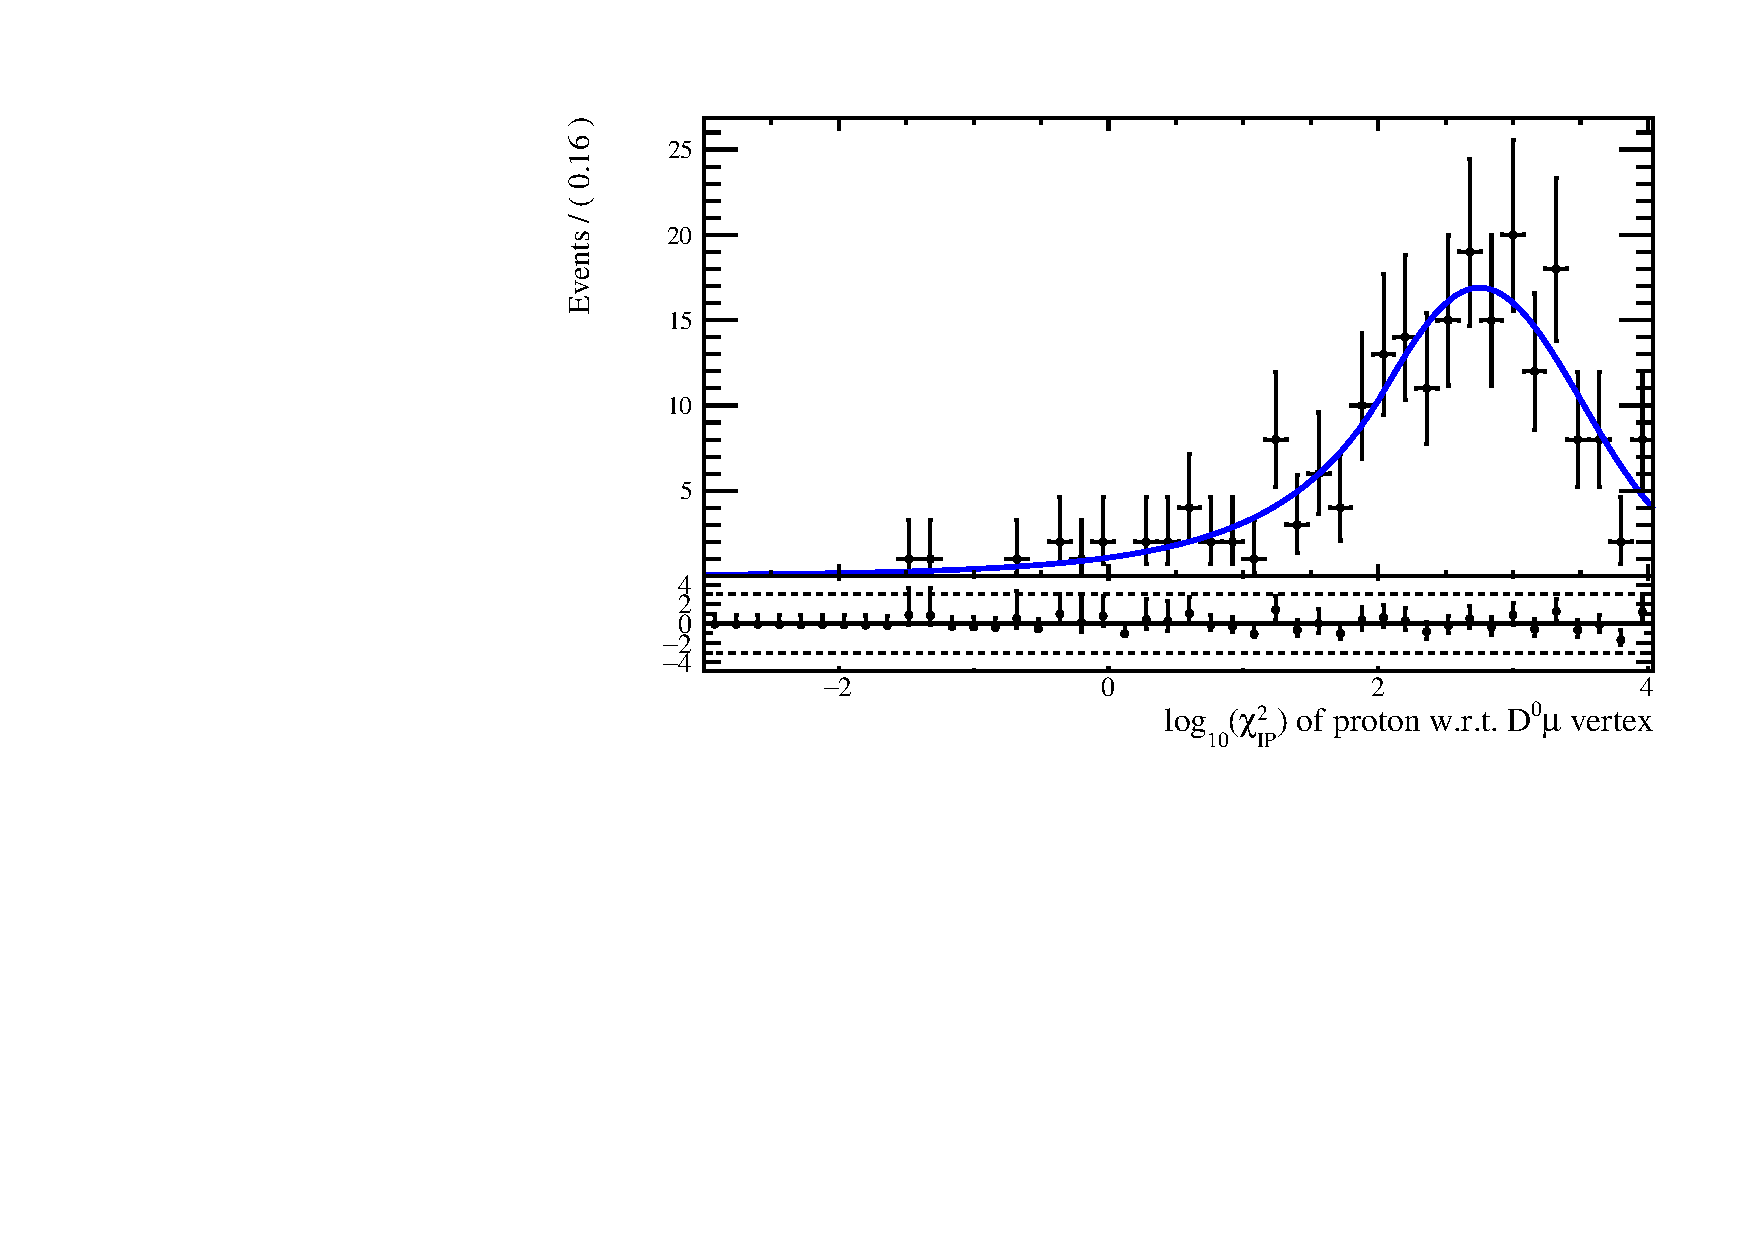
\includegraphics[width=0.75\textwidth]{LbToD0p/fits/MC_B2D0munu_BKG/logIP_RS/fit_CB}
	\caption{Fit to the (RS and WS added) \logIP shape of the background simulation.
             The distribution is modeled with a CrystalBall function.}
    \label{fig:fit_logIP_MC_BKG}
\end{figure}

\subsection{One-dimensional fit to the \logIP distribution in data}
\label{sec:ControlLogIP}
To control if the chosen parametrization of the \logIP distribution gained from simulation describes data, a one-dimensional \logIP-fit on data is performed.
For that purpose, the double bifurcated Gaussian as signal component and the CrystalBall as background component are added, i.e. the total probabiltiy density function $\mathcal{P}$ for that fit is:
\begin{align}
    &\mathcal{P}(x|N_\text{sig}, N_\text{bkg}, x_{0, \text{sig}}, x_{0, \text{bkg}} \vec{\sigmaL{}}_{,\text{sig}}, \vec{\sigmaR{}}_{,\text{sig}}, f_{\BfG_1}, \sigma_\text{bkg}, \alpha, n) \propto \nonumber\\
    &N_\text{sig} \DBfG(x|x_{0, \text{sig}}, \vec{\sigmaL{}}_{,\text{sig}}, \vec{\sigmaR{}}_{,\text{sig}}, f_{\BfG_1}) + N_\text{bkg} \CB(x| x_{0, \text{bkg}}, \sigma_\text{bkg}, \alpha, n)
\end{align},
where $N_\text{sig}$ denotes the signal yield and $N_\text{bkg}$ the background yield respectively.
The fitresult can be seen in Figure \ref{fig:fit_logIP_RS} and the corresponding yields and parameter values are listed in Table \ref{tab:logIP_RS}.
\begin{figure}[ptb]
    \centering
	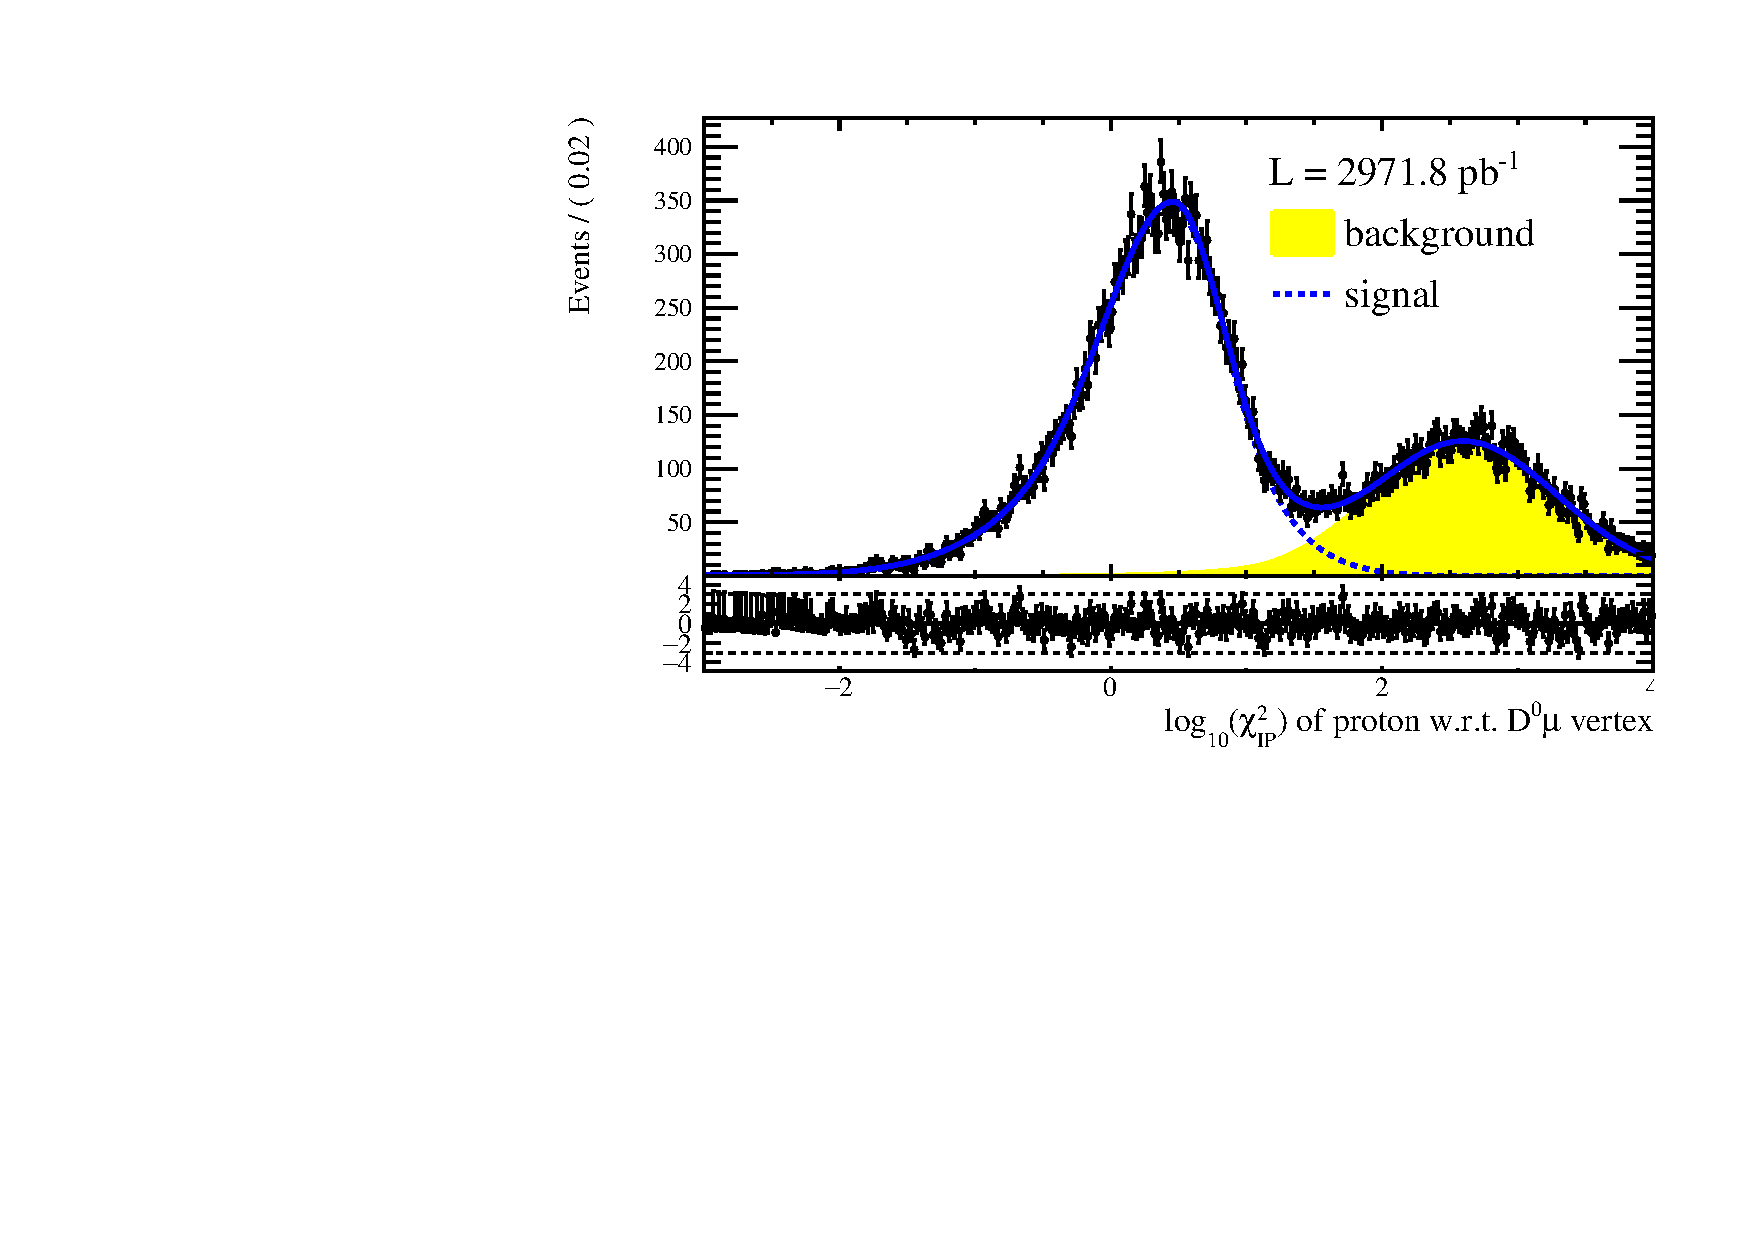
\includegraphics[width=\textwidth]{LbToD0p/fits/data/logIP_RS/fit_DBfG_CB}
	\caption{\logIP distribution of the data sample.
             A binned likelihood fit is performed on it with the sum of a double bifurcated Gaussian for the signal (blue, dashed line) and a CrystalBall function for the background component (yellow shaded). }
    \label{fig:fit_logIP_RS}
\end{figure}
 
\begin{table}[h]
    \centering
    \caption{Results of the onedimensional \logIP fit on data.}
    \label{tab:logIP_RS}
    $\begin{array}{lr@{\pm}l}
    \hline
    \text{Variable} & \multicolumn{2}{c}{\text{Value}} \\
    \hline
        \multicolumn{3}{l}{\text{\textbf{Yields}}} \\
\text{signal yield}&(2.325 & 0.028) \cdot 10^{4}\\
\text{background yield}&(1.086 & 0.026) \cdot 10^{4}\\
\multicolumn{3}{l}{\text{\textbf{Signal (\DBfG)}}} \\
\text{mean}&(4.59 & 0.26) \cdot 10^{-1}\\
\text{left width 1}&(8.72 & 0.56) \cdot 10^{-1}\\
\text{right width 1}&(5.74 & 0.44) \cdot 10^{-1}\\
\text{left width 2}&(4.72 & 0.55) \cdot 10^{-1}\\
\text{right width 2}&(3.37 & 0.23) \cdot 10^{-1}\\
\text{fraction BfG 1}&(5.61 & 0.89) \cdot 10^{-1}\\
\multicolumn{3}{l}{\text{\textbf{Background (\CB)}}} \\
\text{CB mean}&(2.6 & 0.017) \cdot 10^{0}\\
\text{CB $\sigma$}&(6.85 & 0.14) \cdot 10^{-1}\\
\text{CB $\alpha$}&(2.035 & 0.099) \cdot 10^{0}\\
\text{CB $n$}&(1.62 & 0.45) \cdot 10^{0}\\

\hline
\end{array}$
\end{table}
    

The chosen model very nicely describes the data as can be seen in the pull distribution.
Thus the chosen parametrisation for the \logIP shape is reasonable.
This fit is later also used for systematic studies, since it is already able to distinguish between signal and background yields, see Chapter \ref{sec:Selection} for further discussions.

\subsection{\Dz\proton mass shape}
\label{sec:Shape_mD0p}
To get an idea of the (combinatorial) background shape in the \Dz\proton mass distribution, events with a wrong sign proton, i.e. events with \Dz\antiproton\mun in the final state are used since the transition from \Lb to a \Dz\antiproton\mun final state is physically forbidden by charge
conservation and should thus give a good proxy for randomly combined \LbToDpmunu candidates. 
The \MDp distribution of these wrong sign events is shown in Figure \ref{fig:fit_mD0p_WS} and modeled with an empirical background function
\begin{align}
    \text{EBG}(m|m_0, m_1, m_2, p,c_1) = \text{PS}(m|m_1,m_2) \cdot (m - m_0)^p \cdot \exp\left[ c_1 \left(1-\frac{m_0}{m}\right)\right], \label{eq:EBG}
\end{align}
where $m_0 := m_1 + m_2$ denotes the kinematic \Dz\proton mass threshold and PS the phase space function
\begin{align}
    \text{PS}(m|m_1,m_2) = \frac{1}{2m} \sqrt{\left[m^2 - (m_1 + m_2)^2\right] \left[m^2 - (m_1 - m_2)^2\right]}. \label{eq:PS}
\end{align}
Here and in the following fits, $m_1$ and $m_2$ are fixed to the \Dz respectively proton PDG mass values.
Figure \ref{fig:fit_mD0p_WS} shows the result of the fit.
Again, the model nicely describes the distribution.
It should be noted here, that there is no structure observed in this wrong sign mass spectrum.
This is a good confirmation, that the identification of the two peaks in the \Dz\proton mass for right sign events as \LcResI and \LcResII is appropiate.
\begin{figure}[ptb]
    \centering
	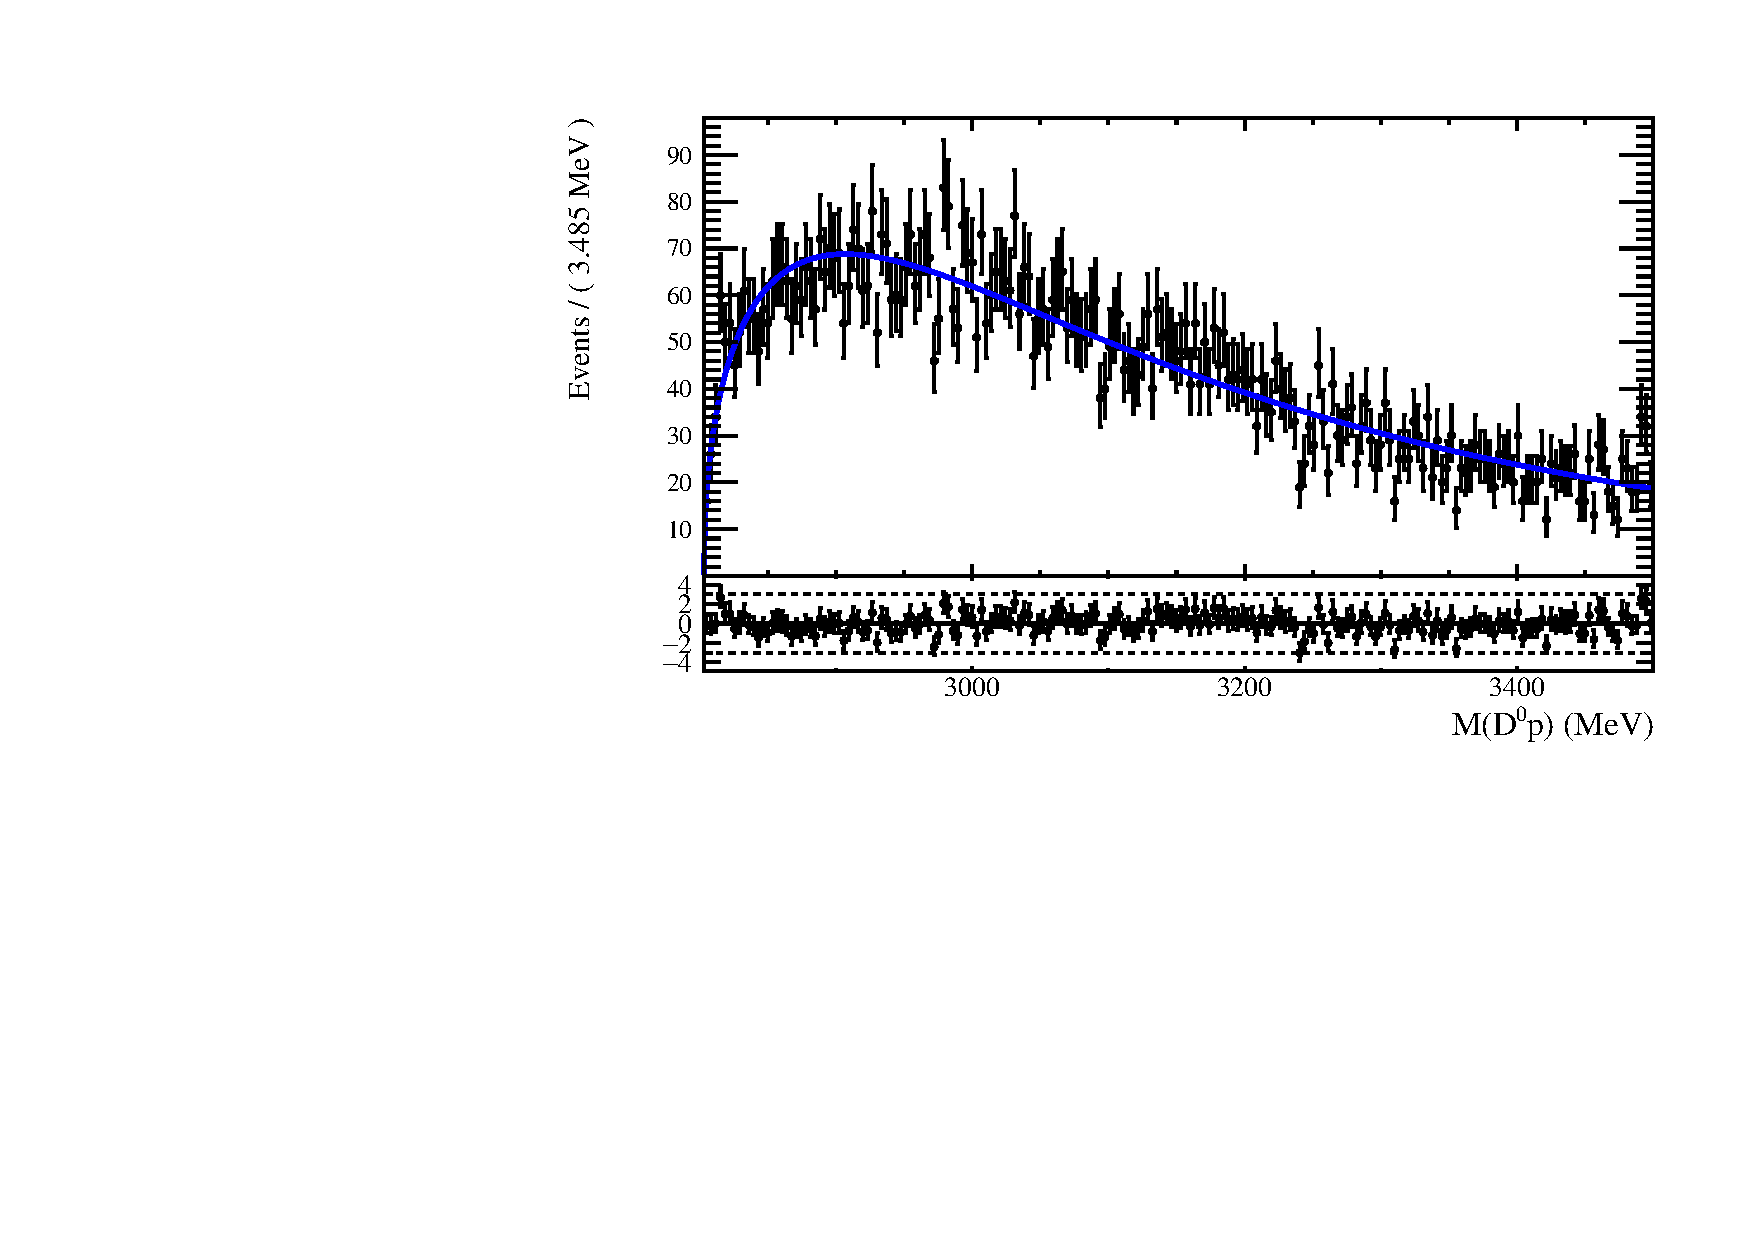
\includegraphics[width=0.75\textwidth]{LbToD0p/fits/data/mD0p_WSp/fit_EmpiricBG}
	\caption{Fit to \Dz\proton mass of wrong sign proton events.
             As model an empiric background function has been chosen, see equation (\ref{eq:EBG})}
    \label{fig:fit_mD0p_WS}
\end{figure}

Unfortunately, there is no reliable simulation predicting the mass shape for the \Dz\proton invariant mass. 
A shape for the signal therefore has to be determined empirically on data. 
A fit to the \Dz\proton mass distribution is applied with the requirement that the \Dz\proton\muon system makes a good vertex, i.e. $\logIP < 1$.
It is shown in Figure \ref{fig:fit_mD0p_RS} top.
This hard requirement strongly suppresses combinatorial background and allows to determine the signal distribution.
As already stated before, the main part of the signal will be nonresonant.
Besides that it is expected to see the two \LcResI and \LcResII resonances.
They are parametrised by a relativistic Breit-Wigner distribution convoluted with a double Gaussian to account for the detector's mass resolution.
The relativistic Breit-Wigner distribution is defined as follows:
\begin{align}
    \text{RelBW}(m|m_R, m_1, m_2, \Gamma_0) \propto 
    \frac{m \Gamma(m|m_R, m_1, m_2, \Gamma_0)}{(m^2-m_R^2)^2 + (m_R \Gamma(m|m_R, m_1, m_2, \Gamma_0))^2}, \label{eq:RelBW}
\end{align}
with 
\begin{align}
    \Gamma(m|m_R, m_1, m_2, \Gamma_0) = \Gamma_0 \frac{m_R}{m} \frac{\PS(m| m_1, m_2)}{\PS(m_R| m_1, m_2)}, 
\end{align}
where PS denotes the phase space function of equation (\ref{eq:PS}), $m_R$ the resonance's mass and $\Gamma_0$ its width \cite{Lb_FF}.
Thus, each resonance is modeled with
\begin{align}
    &\text{RES}(m| m_R, m_1, m_2, \Gamma_0, \sigma_1, \sigma_2, f_1) \propto \nonumber \\
    &\text{RelBW}(m| m_R, m_1, m_2, \Gamma_0) \otimes \left[f_1 \mathcal{G}(m|0,\sigma_1) + (1-f_1) \mathcal{G}(m|0,\sigma_2) \right] \label{eq:RES}
\end{align}
The determination of the mass resolution is thoroughly described in section \ref{sec:Massresolution}. 
The obtained resolution will be fixed in all fits later.

The non-resonant signal part is modeled with the sum of two exponential functions multiplied by a turn-on function.
\begin{align}
    \text{TDExp}(m|m_0, c_0, c_1, c_2, f_{c_1}) \propto \left( 1 - \mathrm{e}^{c_0(m-m_0)} \right) \cdot \left[ f_{c_1} \mathrm{e}^{c_1m} + (1-f_{c_1}) \mathrm{e}^{c_2m} \right]. \label{eq:TDExp}
\end{align}
The turn-on factor is needed to model the steep rise at the \Dz\proton mass threshold.

The fit to the invariant \Dz\proton mass distribution that is shown on the upper side of Figure \ref{fig:fit_mD0p_RS} does not describe the data at low \Dz\proton mass.
Different models for the non-resonant component have been tried to describe this steep curvature without success.
However, when adding another resonant component, the fit converges and describes the data well as can be seen on the lower side of Figure \ref{fig:fit_mD0p_RS}.
This additional component will be labeled ``low mass enhancement" throughout the analysis.
Thus, the total fit function consists of four parts: 
The non-resonant part modeled with the ``turn-on double exponential" function TDExp of eq. (\ref{eq:TDExp}) and relativistic Breit-Wigner functions according eq. (\ref{eq:RES}) for the \LcResI, \LcResII and the low mass enhancement. 
The fit results can be seen in Figure \ref{fig:fit_mD0p_RS} (right) and Table \ref{tab:fit_mD0p_RS}.

Note that at this point, the additional resonant component, the low mass enhancement, is merely introduced to enable the fit to converge and match the data.
There are several possible reasons for such an enhancement.
Nonetheless there is some motivation to choose a resonant model as additional component:
On the one hand the peak looks similar to the other resonances.
On the other hand, there is a similar peak seen in other analyses e.g. \babar is discussing a (much less pronounced) peak at an invariant \Dz\proton mass of about 2840\mev in its study on the \Dz\proton final state in \cite{BaBar_D0p}.
The reason for this peak is not understood so far and is currently studied in different ongoing \lhcb analyses.
Besides some detector effects, backgrounds or kinematical reflections it is not excluded that a new particle is seen here.
A thorough discussion, if this additional component is actually needed and what might cause this peak follows in section \ref{sec:Structure}.
In the following this component is treated as signal since it appears very clear when requiring $\logIP < 1$, i.e. in the background suppressed region making a good decay vertex.
\begin{figure}[ptb]
    \centering
	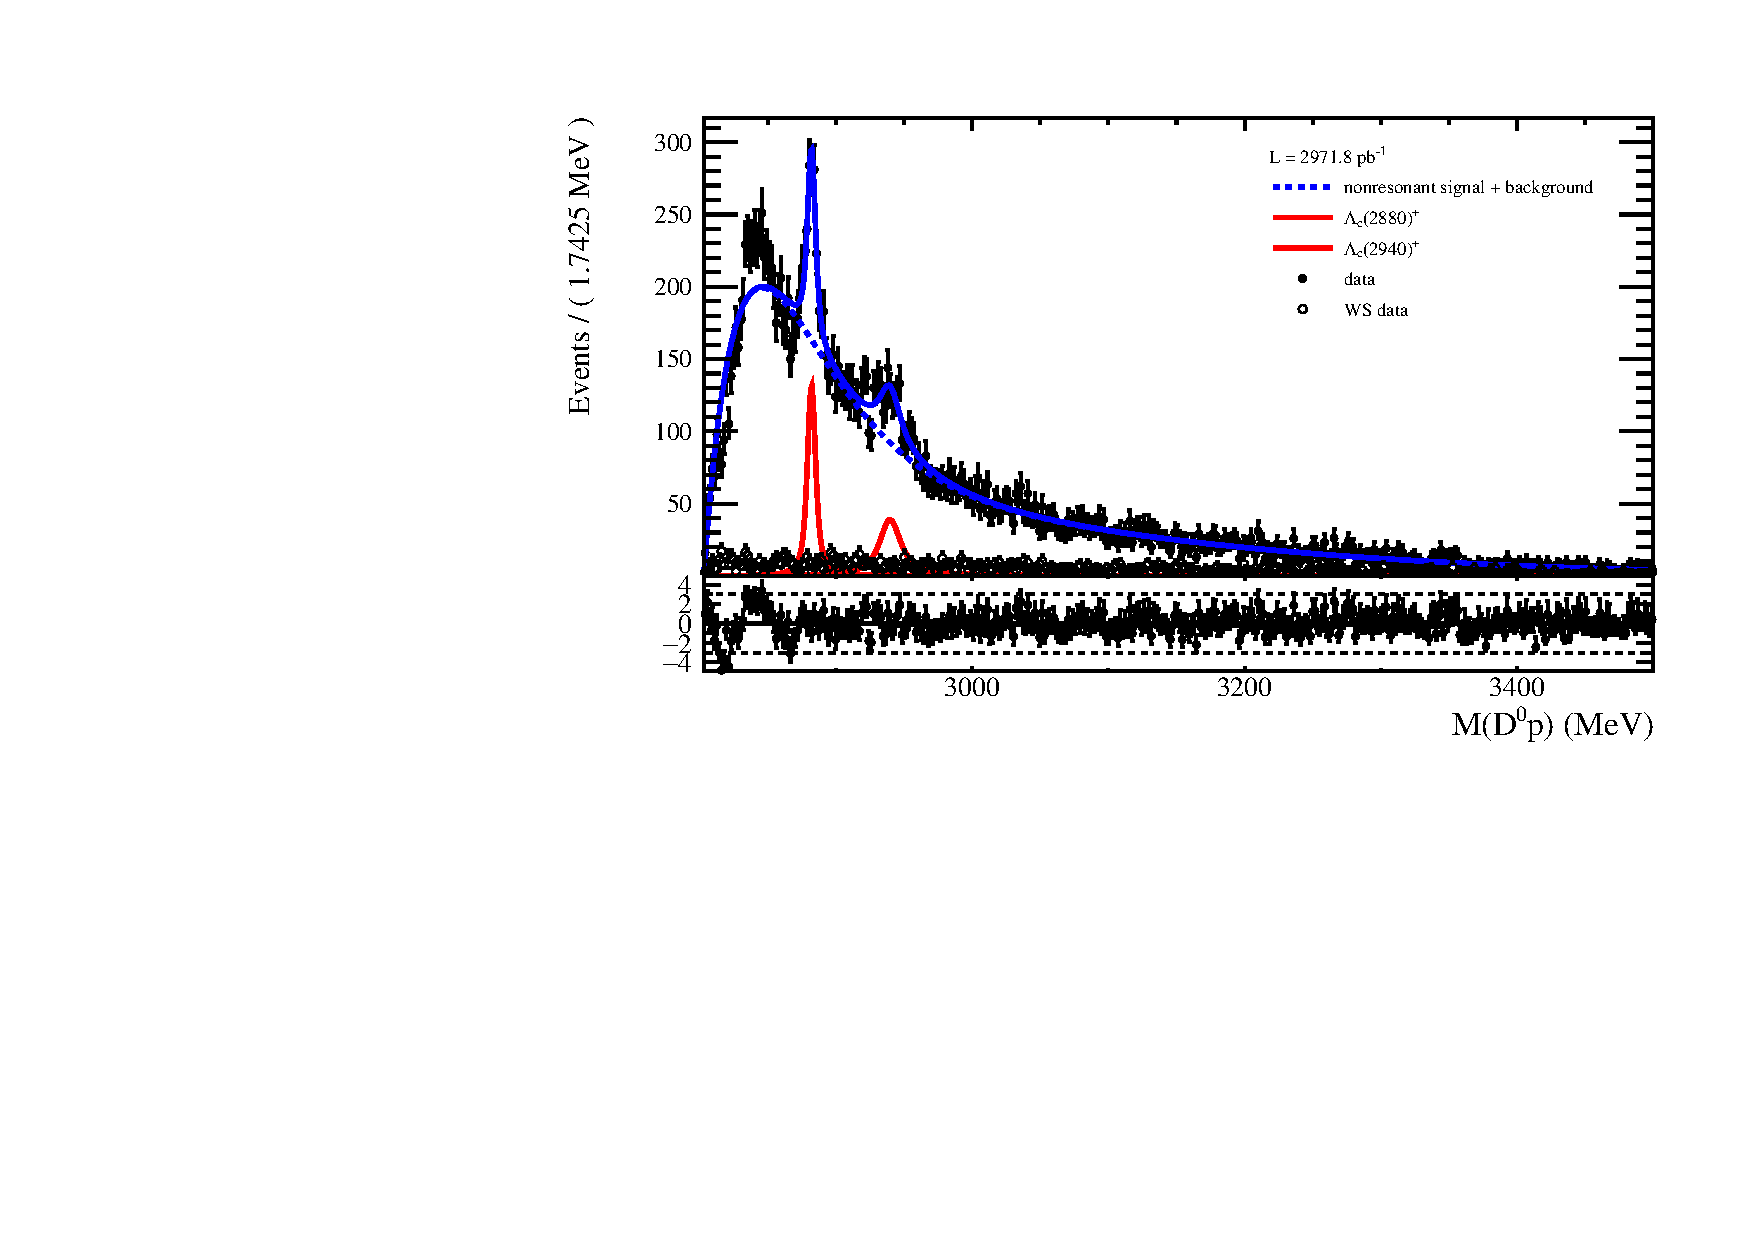
\includegraphics[width=\textwidth]{LbToD0p/fits/data/mD0p_RS/fit_TurnOnDExp_2RelBWPSRes} \\
	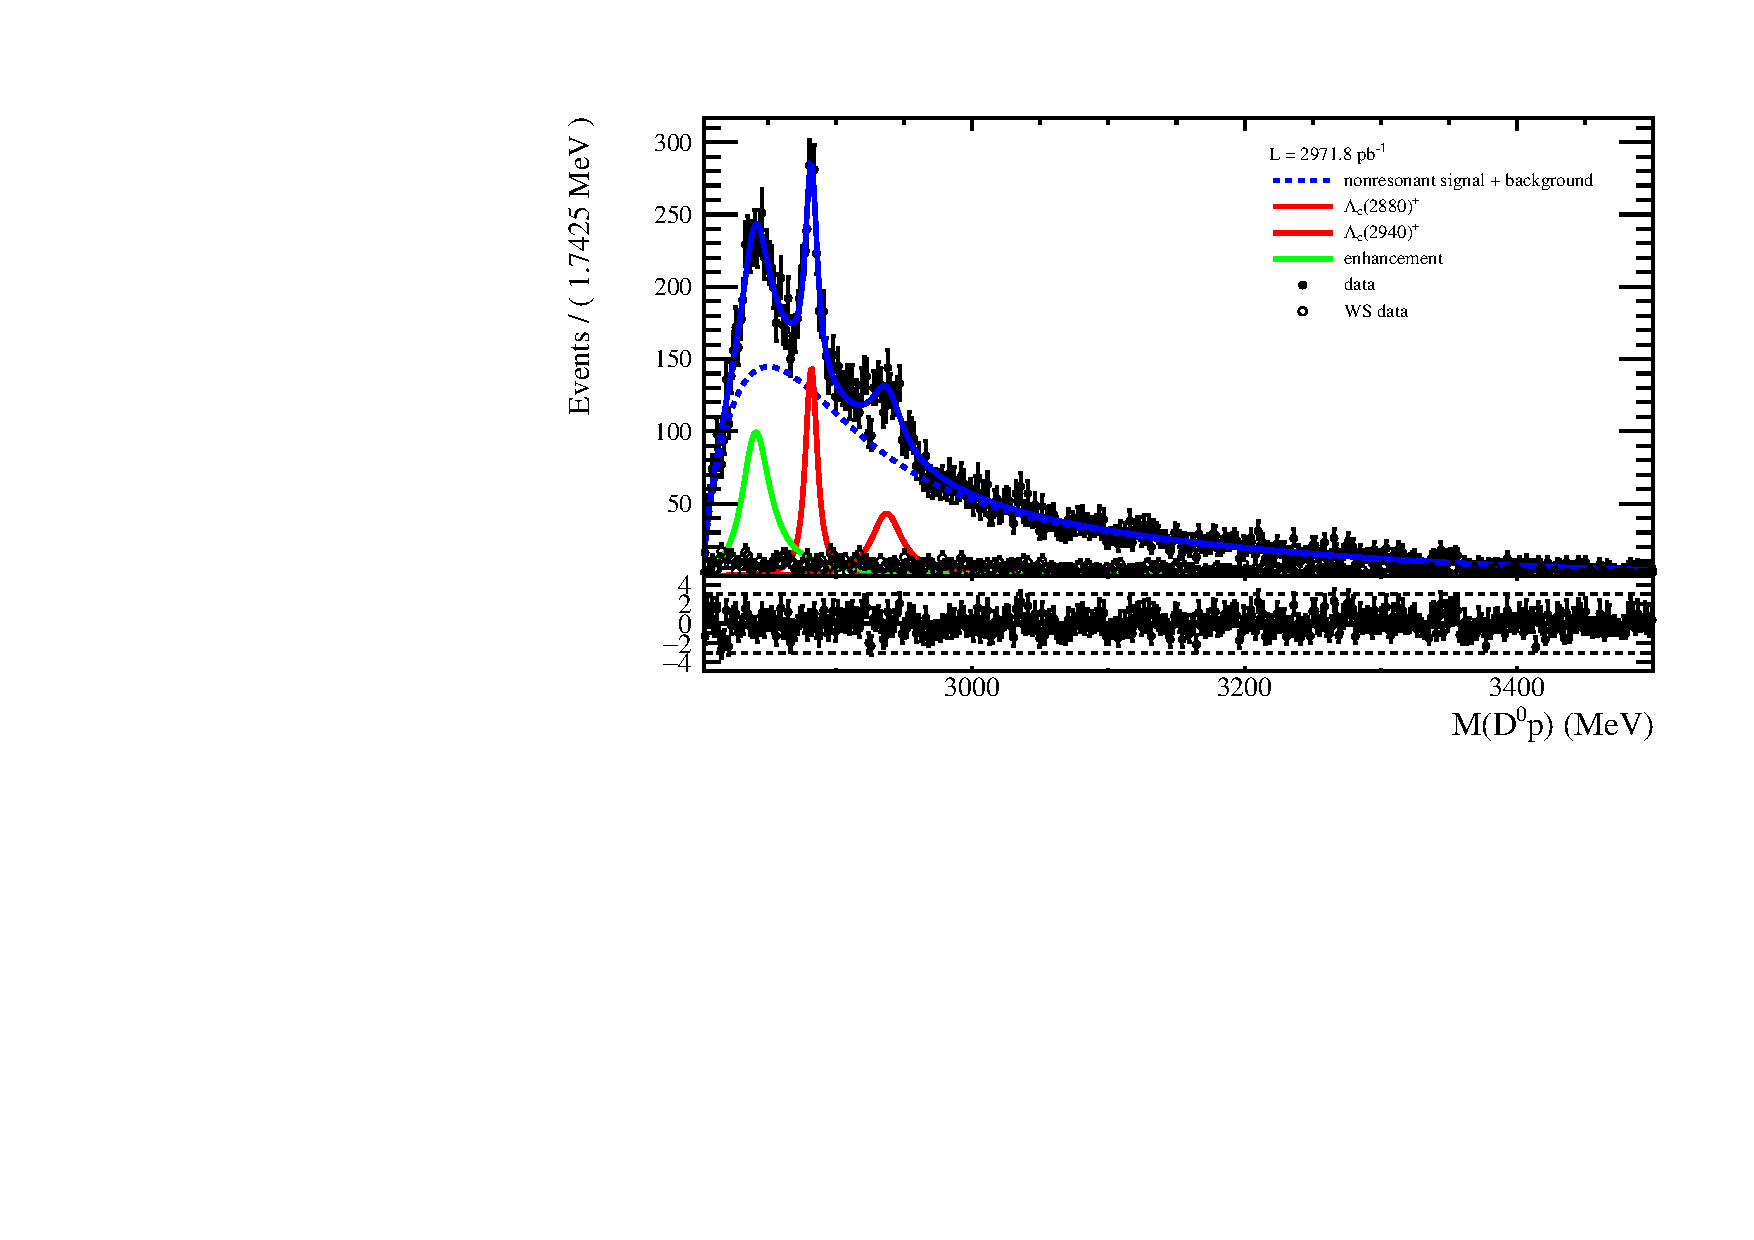
\includegraphics[width=\textwidth]{LbToD0p/fits/data/mD0p_RS/fit_TurnOnDExp_3RelBWPSRes}
	\caption{Invariant \Dz\proton mass distribution when requiring $\logIP < 1$. 
             The upper figure shows a fit with two resonances (red lines) for the \LcResI and \LcResII and a nonresonant part (blue dashed line). 
             Different attempts have been made to get a proper and converging fit, matching the data at low \Dz\proton mass, without success. 
             This issue can be solved by adding an additional resonant component (lower figure, green line), obeying the same fit model like the two resonances.}
    \label{fig:fit_mD0p_RS}
\end{figure}
 
\begin{table}[h]
    \centering
    \caption{Results of the \Dz\proton mass fit.}
    \label{tab:fit_mD0p_RS}
    $\begin{array}{lr@{\pm}l}
    \hline
    \text{Variable} & \multicolumn{2}{c}{\text{Value}} \\
    \hline
        \multicolumn{3}{l}{\text{\textbf{Yields}}} \\
\text{\LcResI signal yield}&(1.26 & 0.16) \cdot 10^{3}\\
\text{\LcResII signal yield}&(1.01 & 0.32) \cdot 10^{3}\\
\text{mass enhancement yield}&(2.12 & 0.44) \cdot 10^{3}\\
\text{nonresonant yield}&(1.65 & 0.08) \cdot 10^{4}\\
\multicolumn{3}{l}{\text{\textbf{\LcResI resonance}}} \\
\text{mean}&(2.88 & 0.00) \cdot 10^{3}\\
\text{width}&(8.90 & 1.40) \cdot 10^{0}\\
\multicolumn{3}{l}{\text{\textbf{\LcResII resonance}}} \\
\text{mean}&(2.94 & 0.00) \cdot 10^{3}\\
\text{width}&(2.62 & 0.79) \cdot 10^{1}\\
\multicolumn{3}{l}{\text{\textbf{Low mass enhancement}}} \\
\text{mean}&(2.84 & 0.00) \cdot 10^{3}\\
\text{width}&(2.44 & 0.37) \cdot 10^{1}\\
\multicolumn{3}{l}{\text{\textbf{nonresonant part}}} \\
\text{turn on mass threshold}&(2.80 & 0.00) \cdot 10^{3}\\
\text{turn on slope}&(-2.00 & 32.00) \cdot 10^{-5}\\
\text{exponential 1 slope}&(-2.34 & 0.13) \cdot 10^{-2}\\
\text{exponential 2 slope}&(-7.07 & 0.20) \cdot 10^{-3}\\
\text{fraction exponential 1}&(7.40 & 0.24) \cdot 10^{-1}\\

\hline
\end{array}$
\end{table}
    

\section{Determination of the mass resolution}
\label{sec:Massresolution}
Due to resolution effects, the width of a resonance in a mass spectrum can appear wider than its natural width.
In this analysis the effect is accounted for by convoluting the Breit-Wigner, which is assumed to be the natural shape of the resonance, with a double Gaussian, describing the smearing of the resonance due to finite mass resolution, see equation (\ref{eq:RES}).

The determination of the mass resolution is performed in a simulation by comparing the generated (also called ``true") mass with the reconstructed mass.
The mean of the mass difference distribution is expected to be zero and the width refers to the mass resolution.
The distribution is described by a double Gaussian function $f_1 \mathcal{G}(m|m_0,\sigma_1) + (1-f_1) \mathcal{G}(m|m_0,\sigma_2)$ to properly describe the broadening of the mass difference distribution in the tails.
To account for a potential mass dependence, this fit is performed in several bins of the true invariant \Dz\proton mass.
The left-hand side of Figure \ref{fig:massresolution} exemplarily shows the mass difference between reconstructed and generated mass together with the fit of a double Gaussian in the bin $2910 < M(\Dz\proton) < 2980 \mev$.
This bin corresponds to the \LcResII resonance.
The fits of all bins can be seen in Appendix \ref{app:Massresolution}, Figure \ref{fig:massresolution_all}.
The widths $\sigma_1$ and $\sigma_2$ and the fraction of the first Gaussian $f_1$ obtained by these fits in the respective bins are used for the parametrisation of the resonances in the nominal \Dz\proton mass fit as described by equation (\ref{eq:RES}).
Table \ref{tab:Massresolution} summarises the obtained values which are used for the further analysis.
Though there is a mass dependence of the resolution over the whole \Dz\proton mass spectrum it is assumed, that the mass resolution can be considered as constant over the natural width of the resonances.
\begin{table}[h]
    \centering
    \caption{Results of the fits to the mass difference distributions for the determination of the mass resolution. Only the values, which are required for the further analysis are quoted here.}
    \label{tab:Massresolution}
    $\begin{array}{lr@{\pm}lr@{\pm}lr@{\pm}l}
    \hline
    \text{Resonant component} & \multicolumn{2}{c}{\sigma_1 [\mev]} & \multicolumn{2}{c}{\sigma_2 [\mev]} & \multicolumn{2}{c}{f_1 [\mev]} \\
    \hline
    \LcResI   & \MassresResIwIval & \MassresResIwIerr & \MassresResIwIIval & \MassresResIwIIerr & \MassresResIfIval & \MassresResIfIerr \\
    \LcResII   & \MassresResIIwIval & \MassresResIIwIerr & \MassresResIIwIIval & \MassresResIIwIIerr & \MassresResIIfIval & \MassresResIIfIerr \\
    \text{enhancement} & \MassresStructurewIval & \MassresStructurewIerr & \MassresStructurewIIval & \MassresStructurewIIerr & \MassresStructurefIval & \MassresStructurefIerr \\
    \hline
    \end{array}$
\end{table}
The right-hand side of Figure \ref{fig:massresolution} shows the root-mean-square of the mass difference distributions in the different bins.
This serves as a measure for the mass resolution and how it evolves since it is hard to assign a single value for the mass resolution due to the fit of a double Gaussian.
At \Dz\proton mass threshold, the \Dz and the proton are at rest.
Thus, the measured \Dz\proton mass is just the sum of the PDG masses of the \Dz and the proton.
Hence, there is no sensitivity to a mass resolution at threshold.
If the measured \Dz\proton mass is above the threshold, there are contributions from the momenta of the \Dz and the proton to the measured \Dz\proton mass, too, influencing the mass resolution.
As the uncertainties of the momenta gets larger for increasing momenta, the mass resolution increases as well.
\begin{figure}[ptb]
    \centering
	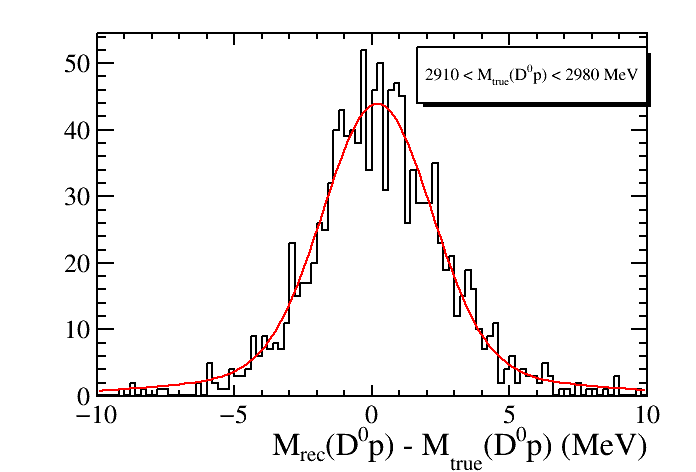
\includegraphics[width=0.49\textwidth]{LbToD0p/massresolution/massresolution_03}
	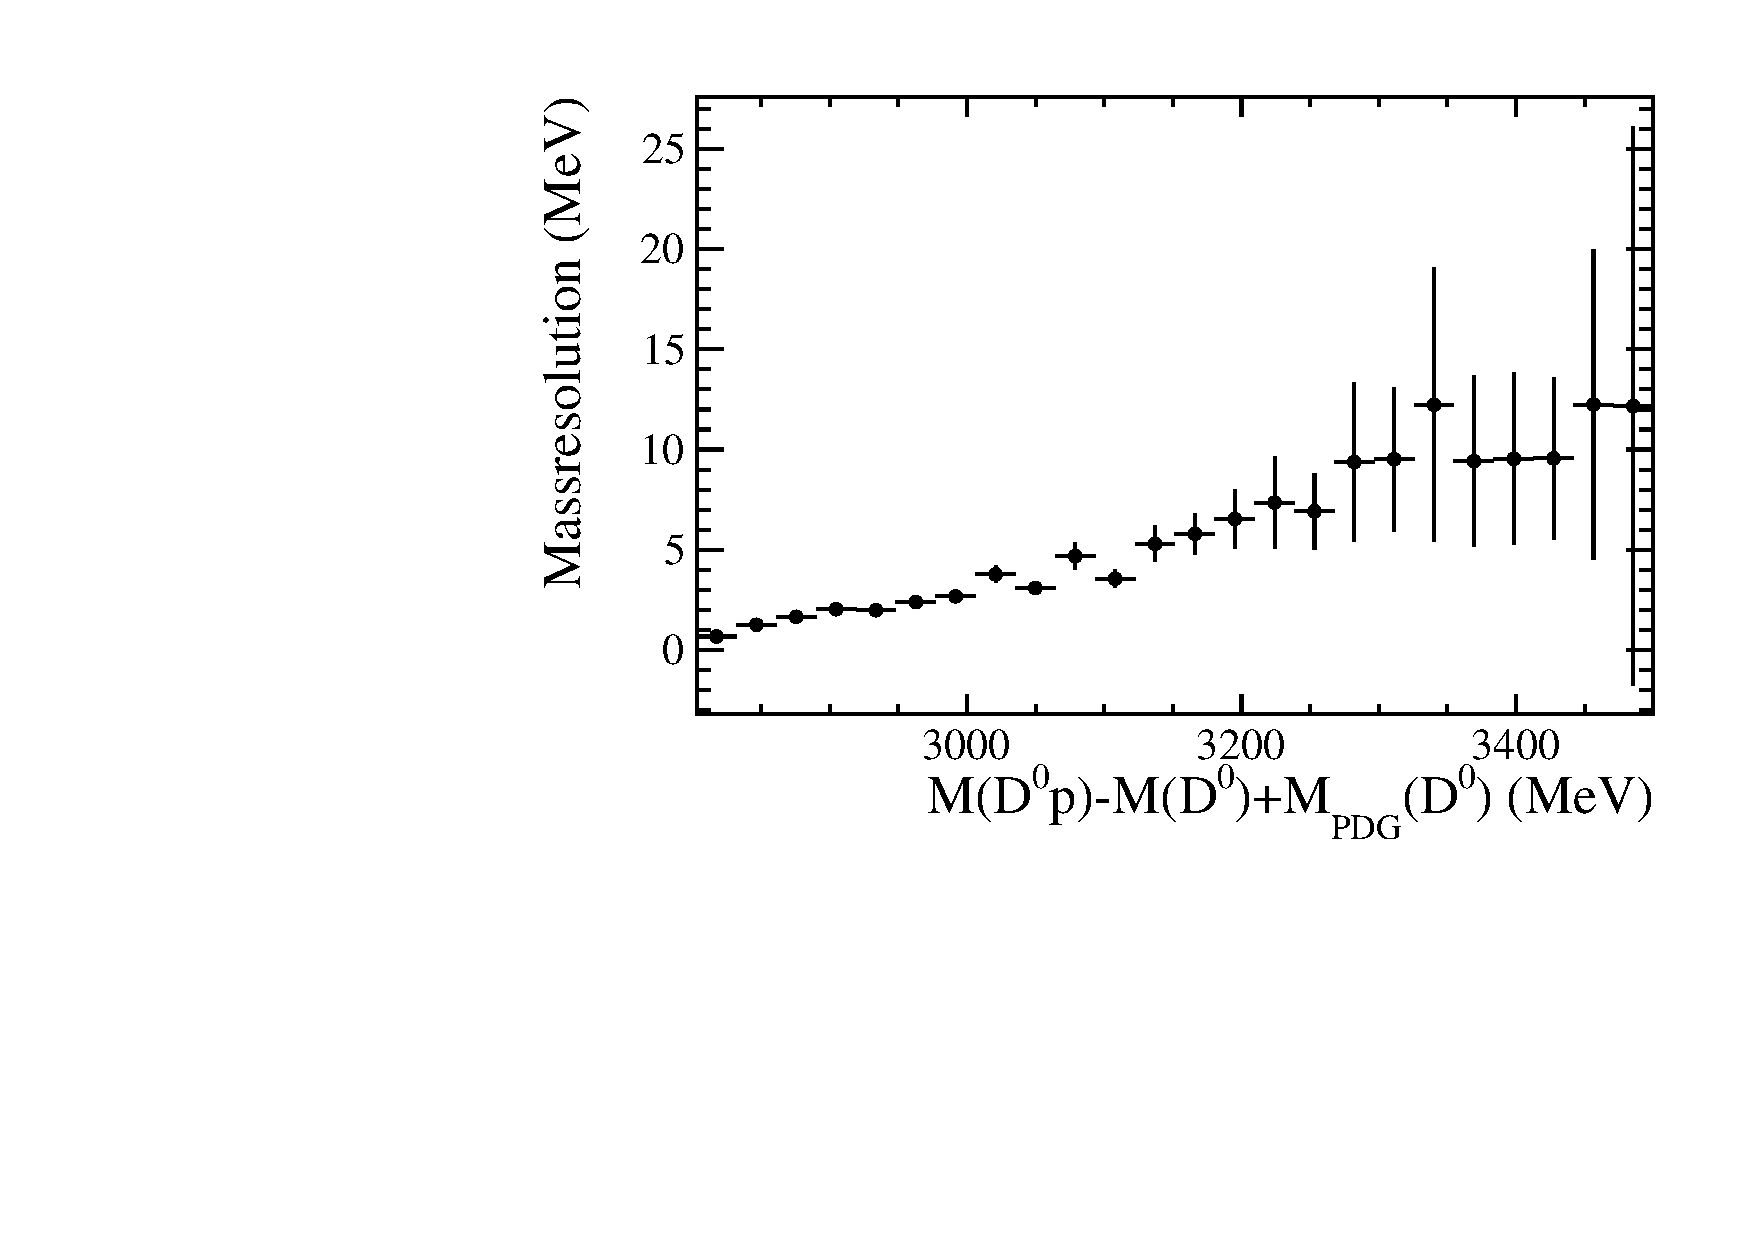
\includegraphics[width=0.49\textwidth]{LbToD0p/massresolution/massresolution_widths}
	\caption{Left: Fit of a Gaussian to the difference between generated and reconstructed \Dz\proton mass of the simulation sample in the range $2910 < M(\Dz\proton) < 2980 \mev$, corresponding to the bin of the \LcResII resonance. Right: root-mean-square (RMS) of the mass difference distributions for each bin.
    The RMS serves as a measure for the mass resolution since it is not easy to assign a single value for the mass resolution, since the distribution is modeled with a double Gaussian.}
    \label{fig:massresolution}
\end{figure}


\section{Nominal fit in two dimensions}
\label{sec:Fit_2D}
With a two-dimensional fit to the \Dz\proton mass and the \logIP distribution it is possible to distinguish between nonresonant signal and background in the \Dz\proton mass spectrum as already explained.
Thus, the different pieces of the previous sections are put together for a fit of both distributions.

It is assumed that the \logIP distribution is the same for all 4 different signal components (non-resonant signal, \LcResI, \LcResII, enhancement), since their decay topologies are the same\footnote{Presumed, that the enhancement indeed emerges to be a resonance or another signal component.}.
Hence, their \logIP distributions share all parameters. 
For the \logIP signal part a double Bifurcated Gaussian \DBfG is chosen, whereas the background is modeled by a CrystalBall function \CB.
The \Dz\proton mass' signal components are modeled with the same parametrisation as described in section \ref{sec:Shape_mD0p}. 
The empiric background function EBG is used to describe the background.
Thus, the total parametrisation $\mathcal{P}_\text{2D}$ of the two-dimensional \logIP/\MDp distribution is
\begin{align}
    & \mathcal{P}_\text{2D}(x, m | \vec{\lambda}) \propto \nonumber \\
    & \DBfG(x|x_{0, \text{sig}}, \vec{\sigma}_{\text{L,sig}}, \vec{\sigma}_{\text{R,sig}}, f_{\BfG_1}) \nonumber \\
    & \quad \cdot \left[\phantom{+} N_\text{nonres} \cdot \text{TDExp}(m|m_0, c_0, c_1, c_2, f_{c_1}) \right. \nonumber \\
    & \quad \phantom{\cdot [} + N_{\LcResI} \cdot \RES(m| m_{\LcResI}, m_1, m_2, \Gamma_{0, \LcResI}, \vec{\sigma}_{\LcResI}, f_{1, \LcResI}) \nonumber \\
    & \quad \phantom{\cdot [} + N_{\LcResII} \cdot \RES(m| m_{\LcResII}, m_1, m_2, \Gamma_{0, \LcResII}, \vec{\sigma}_{\LcResII}, f_{1, \LcResII}) \nonumber \\
    & \quad \phantom{\cdot [} + N_\text{enh} \cdot \RES(m| m_\text{enh}, m_1, m_2, \Gamma_{0, \text{enh}}, \vec{\sigma}_{\text{enh}}, f_{1, \text{enh}})\left.\right] \nonumber \\
    & + \CB(x| x_{0, \text{bkg}}, \sigma_\text{bkg}, \alpha, n) \cdot N_\text{bkg} \cdot \text{EBG}(m|m_0, m_1, m_2, p,c_{1, \text{bkg}}),
\end{align}
where $x$ denotes \logIP, $m$ the invariant \Dz\proton mass, $\vec{\lambda}$ the set of all fit parameters and $N_i$ the yields of the respective components.
All other parameters are explained in the sections before, where the different functions have been introduced.
All parameters are floating except for the mass resolution parameters of the resonant components in \RES(...) and the \Dz and proton mass ($m_1$ respectively $m_2$), that are required in the phase space function PS, which again is part of the relativistic Breit-Wigner and the empiric background function. 
The results of the fit are shown in Table \ref{tab:2Dfit} and the projections can be seen in Figure \ref{fig:fit2D}.
The model very nicely describes the data.
The pull distributions do not show any abnormalities.
A discussion of the result follows in section \ref{sec:Signalyield_D0p}.
\begin{figure}[ptb]
	\centering
	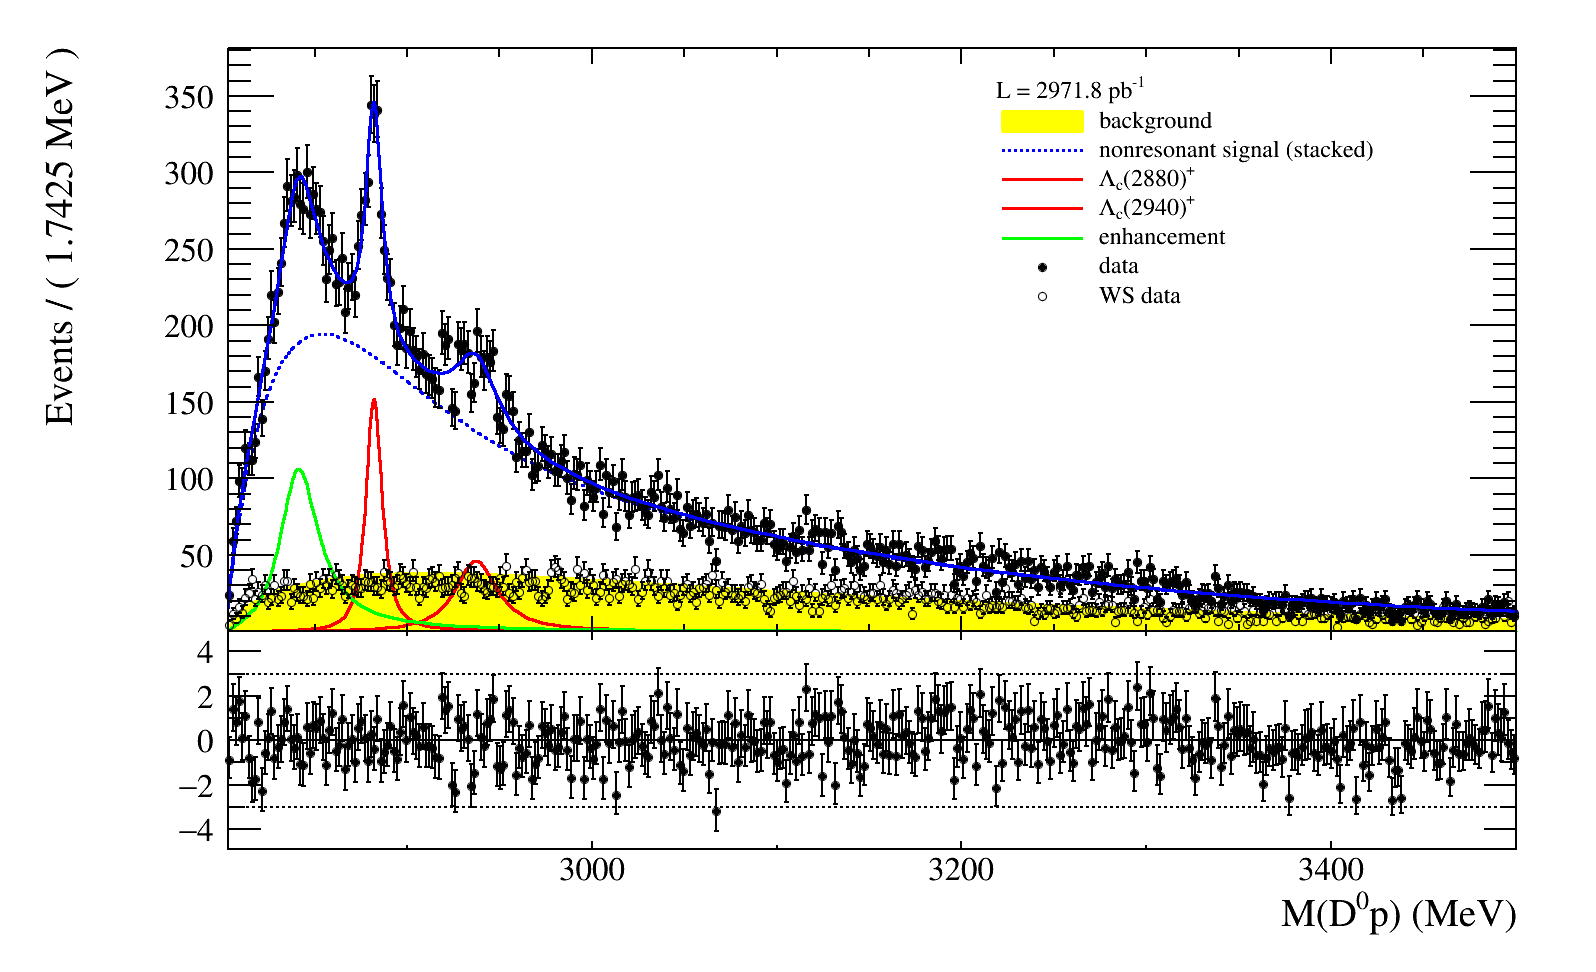
\includegraphics[width=\textwidth]{LbToD0p/fits/data/2Dfit/fit_DBfG_CB_vs_TurnOnDExp_3RelBWPSRes_EmpiricBG_mD0pProj} \\
	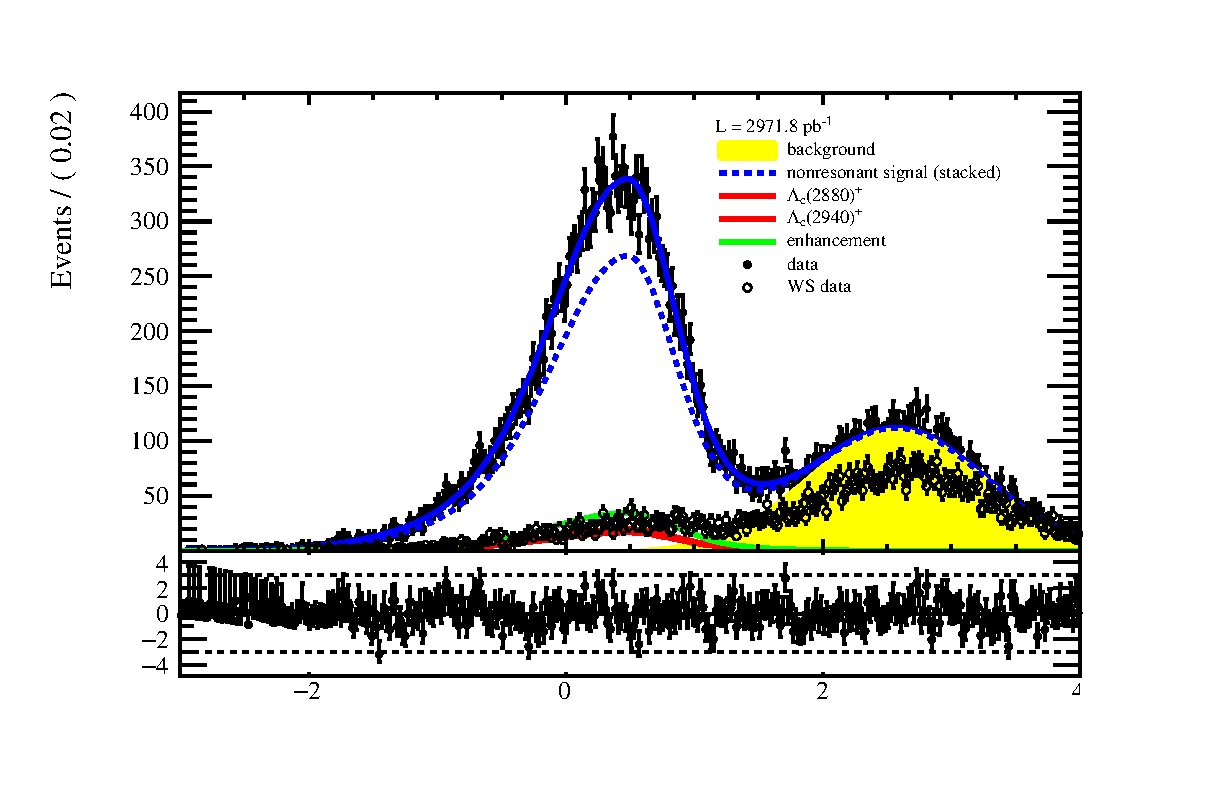
\includegraphics[width=\textwidth]{LbToD0p/fits/data/2Dfit/fit_DBfG_CB_vs_TurnOnDExp_3RelBWPSRes_EmpiricBG_logIPProj}
	\caption{Two-dimensional fit to the \LbToDpmunuX candidates. Top: projection of invariant \Dz\proton mass. Bottom: projection of \logIP distribution projection.
             The fit model is described in the text.
             The yellow shaded area shows the background component, stacked on top the non-resonant signal component marked as blue, dashed line.
             The two identified \LcResI and \LcResII resonances are drawn with a red solid line, the additional enhancement in green.
             For comparison the open circles show the wrong sign events.}
	\label{fig:fit2D}
\end{figure}
 
\begin{table}[h]
    \centering
    \caption{Results of the twodimensional M(\Dz\proton) and \logIP fit.}
    \label{tab:2Dfit}
    $\begin{array}{lr@{\pm}l}
    \hline
    \text{Variable} & \multicolumn{2}{c}{\text{Value}} \\
    \hline
        \multicolumn{3}{l}{\text{\textbf{Yields}}} \\
\text{\LcResI signal yield}&(1.28 & 0.15) \cdot 10^{3}\\
\text{\LcResII signal yield}&(1.06 & 0.24) \cdot 10^{3}\\
\text{mass enhancement yield}&(2.29 & 0.45) \cdot 10^{3}\\
\text{nonresonant signal yield}&(1.83 & 0.069) \cdot 10^{4}\\
\text{background yield}&(9.42 & 0.14) \cdot 10^{3}\\
\multicolumn{3}{l}{\text{\textbf{\LcResI resonance}}} \\
\text{mean [\mev]}&(2.88197 & 0.00034) \cdot 10^{3}\\
\text{width [\mev]}&(7.4 & 1.3) \cdot 10^{0}\\
\multicolumn{3}{l}{\text{\textbf{\LcResII resonance}}} \\
\text{mean [\mev]}&(2.9374 & 0.0016) \cdot 10^{3}\\
\text{width [\mev]}&(2.44 & 0.55) \cdot 10^{1}\\
\multicolumn{3}{l}{\text{\textbf{Low mass enhancement}}} \\
\text{mean [\mev]}&(2.84222 & 0.00088) \cdot 10^{3}\\
\text{width [\mev]}&(2.51 & 0.37) \cdot 10^{1}\\
\multicolumn{3}{l}{\text{\textbf{Nonresonant signal}}} \\
\text{turn on mass threshold [\mev]}&(2.80127 & 0.00057) \cdot 10^{3}\\
\text{turn on slope [\mev$^{-1}$]}&(-2.0 & 36.0) \cdot 10^{-4}\\
\text{exponential 1 slope [\mev$^{-1}$]}&(-2.34 & 0.14) \cdot 10^{-2}\\
\text{exponential 2 slope [\mev$^{-1}$]}&(-7.03 & 0.78) \cdot 10^{-3}\\
\text{fraction exponential 1}&(7.36 & 0.25) \cdot 10^{-1}\\
\multicolumn{3}{l}{\text{\textbf{Background (mass)}}} \\
\text{Empiric BG $c_1$ [\mev$^{-1}$]}&(-1.595 & 0.05) \cdot 10^{1}\\
\text{Empiric BG $p_0$}&(5.6 & 3.0) \cdot 10^{-2}\\
\multicolumn{3}{l}{\text{\textbf{Signal (\logIP)}}} \\
\text{mean}&(4.8 & 0.16) \cdot 10^{-1}\\
\text{left width 1}&(9.76 & 0.27) \cdot 10^{-1}\\
\text{right width 1}&(6.22 & 0.32) \cdot 10^{-1}\\
\text{left width 2}&(5.37 & 0.24) \cdot 10^{-1}\\
\text{right width 2}&(3.41 & 0.15) \cdot 10^{-1}\\
\text{fraction BfG 1}&(4.21 & 0.42) \cdot 10^{-1}\\
\multicolumn{3}{l}{\text{\textbf{Background (\logIP)}}} \\
\text{CB mean}&(2.573 & 0.012) \cdot 10^{0}\\
\text{CB $\sigma$}&(6.87 & 0.11) \cdot 10^{-1}\\
\text{CB $\alpha$}&(7.1 & 3.8) \cdot 10^{0}\\
\text{CB $n$}&(3.0 & 1.4) \cdot 10^{0}\\

\hline
\end{array}$
\end{table}
    

% ==================================
% Subsection: Control of the method
% ==================================
\section{Fit to the wrong sign proton data as cross-check}

As a cross-check the two-dimensionsal fit is performed for the wrong sign data with the same parametrisation as for the right sign data in section \ref{sec:Fit_2D}.
However, due to the absence of resonances it is purely described by the nonresonant functions, i.e. the nonresonant signal component and the background component.
The respective plots can be seen in Figure \ref{fig:fit_2D_WS}. 
No structure in the mass distribution is seen, especially the \LcResI and \LcResII resonances vanish in the wrong sign \Dz\proton.
Interesting is to note, that besides the two resonances even the enhancement vanishes.
Thus, it cannot be explained by random combinations of the particles.
Concerning the \logIP distribution, there is nevertheless a ``signal-like" part. 
This is presumably background from \BToDmunuX decays, where the $X$ is of ``wrong charge" and moreover misidentified as (anti)proton.
Since the physics are different for right sign and wrong sign events, the yield obtained in this WS fit cannot easily be subtracted from the nominal fit to account for fake proton backgrounds.
A more thorough study on fake backgrounds will be performed in Chapter \ref{sec:Backgrounds}.
\begin{figure}[ptb]
	\centering
	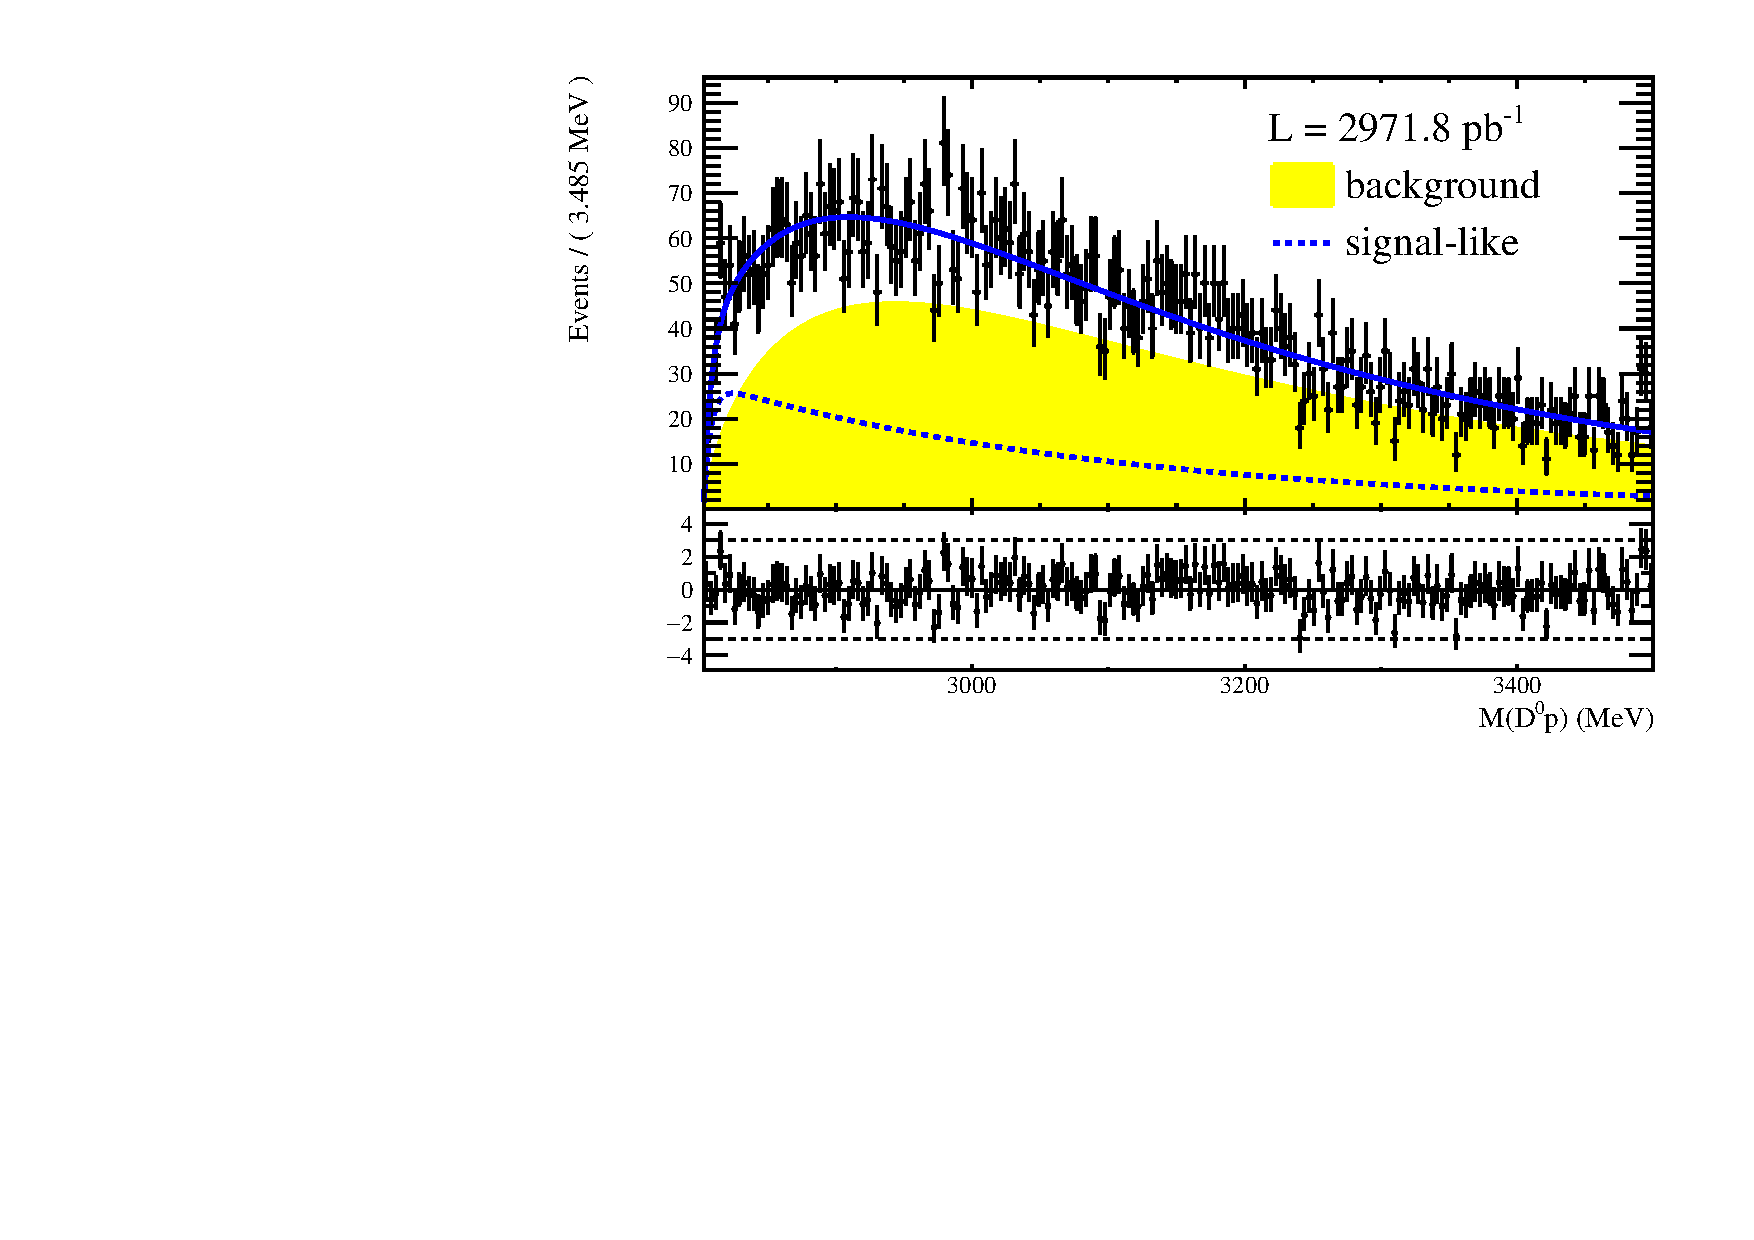
\includegraphics[width=0.49\textwidth]{LbToD0p/fits/data/2DWSfit/fit_DBfG_CB_vs_TurnOnDExp_EmpiricBG_mD0pProj}
	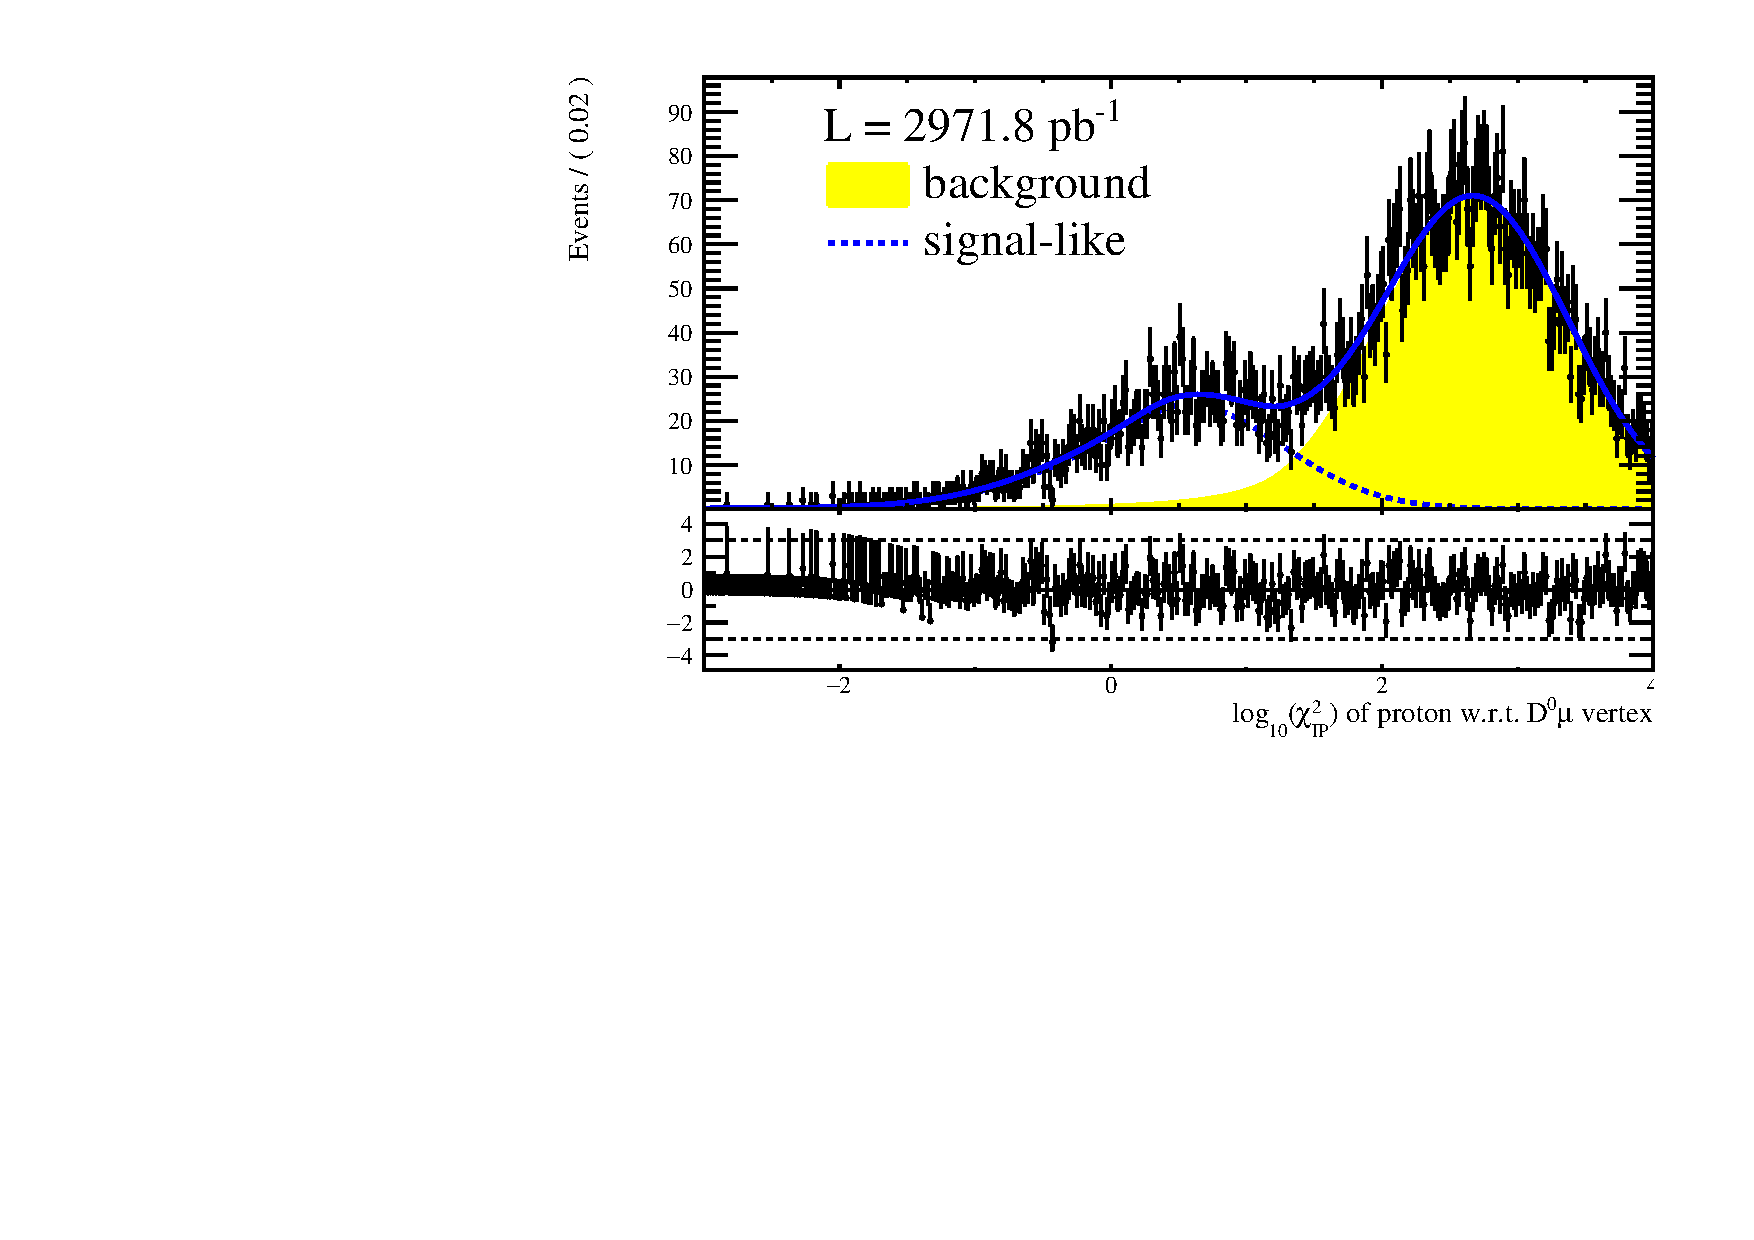
\includegraphics[width=0.49\textwidth]{LbToD0p/fits/data/2DWSfit/fit_DBfG_CB_vs_TurnOnDExp_EmpiricBG_logIPProj}
	\caption{Invariant \Dz\proton mass (left) and \logIP (right) distribution for ``wrong sign" (WS) events.
             The signal-like component (blue, dashed line) of the fit can be assigned to \BToDmunuX decays, where the $X$ is a fake proton of ``wrong" charge.}
	\label{fig:fit_2D_WS}
\end{figure}


% ==================================
% Section: Signal yield and resonances
% ==================================
\section{Extraction of \LbToDpmunuX signal yield together with \LcResI and \LcResII properties}
\label{sec:Signalyield_D0p}
From the previous fits different results can be obtained. 
The most important result is the \LbToDpmunuX signal yield \NDp for the determination of \R.
This result is obtained by the nominal two-dimensional fit.
The obtained yields for the non-resonant component, the \LcResI and the \LcResII as well as the enhancement, which can be found in Table \ref{tab:2Dfit} are summed up.
Thus, the total \LbToDpmunuX signal yield is
\begin{align*}
    \NDp &= N_{\text{nonres}} + N_{\LcResI} + N_{\LcResII} + N_{\text{enh}} \\
         &= (\NDpvalscient \pm \NDperrscient)\cdot 10^{\NDpexpscient}. 
\end{align*}
Remember, that the aim of this thesis is to measure the inclusive branching ratio of \LbToDpmunuX.
That is why all components ending up in a final state containing a \Dz, a proton and a muon are taken summed up for the total signal yield.
Again, it has to be confirmed in chapter \ref{sec:Structure}, that it is appropriate to consider the enhancement as signal.

As a side effect, the properties of the \LcResI and \LcResII resonances are extracted from the fit of the invariant \Dz\proton mass.
In this case it is not needed to distinguish between nonresonant signal and background, since only the peaks are of interest. 
To avoid uncertainties caused by this distinction, the properties of the two resonances are taken from the one-dimensional fit to the invariant \Dz\proton mass (see Table \ref{tab:fit_mD0p_RS}):
\begin{align*}
    \LcResI: \qquad  m_{\LcResI}       &= (\LcResImeanval \pm \LcResImeanerr) \mev, \\
                     \Gamma_{\LcResI}  &= (\LcResIwidthval \pm \LcResIwidtherr) \mev, \\
    \LcResII: \qquad m_{\LcResII}      &= (\LcResIImeanval \pm \LcResIImeanerr) \mev, \\
                     \Gamma_{\LcResII} &= (\LcResIIwidthval \pm \LcResIIwidtherr) \mev.
\end{align*}
The PDG values for the properties of the two resonances are $m_{\LcResI, \text{PDG}} = (2881.53 \pm 0.35)\mev$ and $\Gamma_{\LcResI, \text{PDG}} = (5.8 \pm 1.1)\mev$ for the \LcResI as well as $m_{\LcResII, \text{PDG}} = (2939.3^{+1.4}_{-1.5})\mev$ and $\Gamma_{\LcResII, \text{PDG}} = (17^{+8}_{-6})\mev$ for the \LcResII respectively.
These values are based on a \babar measurement of the \Dz\proton final state and a \belle measurement of \LcResI/\LcResII decays into $\Sigma_\cquark(2455)^{0,++}\pipm$ \cite{Belle_LcRes}.
The obtained results are in good agreement with the current world averages.

Though the reason for the low mass enhancement is not understood so far and it cannot be concluded if a new particle is seen, the obtained mass and width should be quoted here for the sake of completeness:
\begin{align*}
    \text{enhancement}: \qquad  m_{\text{enh}} &= (\Structuremeanval \pm \Structuremeanerr) \mev, \\
                                \Gamma_{\text{enh}}   &= (\Structurewidthval \pm \Structurewidtherr) \mev.
\end{align*}
